% Chapter pd: the note of October 5, 2026, assembled for the compendium -- do not edit by hand
\chapter{Detailed derivation of the quantum theory of inverse bremsstrahlung heating of the free electrons of a plasma}\label{pd:chapter}
\notedate{October 5, 2026}
\begingroup
\noindent\emph{These notes derive, with every intermediate result written
out, the rate at which a laser field heats the free electrons of a fully
ionized plasma by inverse bremsstrahlung. The starting point is the
Schr\"odinger equation of an electron in the field of the laser and of the
ions. The electron in the laser field is described exactly by the Volkov
states \cite{pd:Volkov1935}, the ion potential is treated in Born approximation
as in Bunkin and Fedorov \cite{pd:BunkinFedorov1966}, and the occupation numbers
obey a kinetic equation that is derived with the operator method of the
quantum Boltzmann equation paper \cite{pd:Watson2026}. The classical treatment
of Atzeni and Meyer-ter-Vehn \cite{pd:Atzeni2004} is the baseline. Every boxed
result is checked numerically by a script, which Appendix~\ref{pd:app:checks} describes.}

\medskip
\noindent For notation, Gaussian units are used throughout, as in
\cite{pd:Atzeni2004}. The electron has charge $-e$ and mass $m$. The ions have
charge $Ze$, are infinitely heavy and sit at fixed positions $\Rv_j$ with
density $n_i$, and the plasma is neutral, $n_e=Zn_i$. The temperature $T$ is
in kelvin and $\kB$ is written explicitly. The laser field is uniform and
linearly polarized along the unit vector $\ehat$. The electrons are in a box
of volume $\Vol$ with periodic boundary conditions, a momentum transfer is
written $\hbar\kv$, and the integer $\ell$ counts the photons absorbed in one
collision, with $\ell<0$ for emission. The mean occupation of the electron
state of momentum $\pv$, per spin state, is $f_{\pv}$. It is the $n_{\pv}$ of
the quantum Boltzmann equation paper. The Fourier transform of a function of
position is $\tilde v(\kv)=\int v(\rv)\,e^{-i\kv\cdot\rv}\,\dd^3r$. A term
that is struck through vanishes, for the reason given at that step. A boxed
equation is a result that is used later. An equation of another document is
cited by its own number followed by the reference, as in
Eq.~(11.12)~\cite{pd:Atzeni2004}, and an equation number without a reference is
one of these notes.



\section{Why a quantum theory of inverse bremsstrahlung?}
\label{pd:sec:why}
{\noindent}(1) Inverse bremsstrahlung is the absorption of laser photons by
free electrons while they collide with ions. In laser-driven inertial fusion it
is the preferred absorption mechanism, because the absorbed energy goes into
the thermal electrons and stays where it was absorbed
\cite[Sec.~11.2]{pd:Atzeni2004}.

{\noindent}(2) A free electron alone cannot absorb a photon. Let an electron of
momentum $\pv$ absorb a photon of energy $\hbar\omega$ and momentum
$\hbar\kv_L$. Conservation of energy and momentum requires
\begin{equation}
\frac{|\pv+\hbar\kv_L|^2}{2m}-\frac{p^2}{2m}=\hbar\omega
\quad\Longrightarrow\quad
\frac{\omega}{k_L}=\frac{\pv\cdot\hat\kv_L}{m}+\frac{\hbar k_L}{2m}.
\label{pd:eq:free-absorption}
\end{equation}
The left side is the phase velocity of the transverse wave. In a plasma it is
$c/n_r$ with the refractive index $n_r=(1-\omega_p^2/\omega^2)^{1/2}<1$, so it
exceeds $c$. The right side is the velocity of a nonrelativistic electron
plus $\hbar k_L/2m=\hbar\omega n_r/(2mc)$, which is of order $10^{-5}c$ for
optical photons. The two sides cannot be equal, and a third body has to take
up the momentum. In a fully ionized plasma that body is an ion.

{\noindent}(3) In the classical theory \cite[Sec.~11.1.1]{pd:Atzeni2004} the
electrons oscillate in the laser field and a friction force $-\nu_e m\vv$
represents their collisions with the ions. The absorption coefficient follows
from the imaginary part of the dielectric function, and $\nu_e$ is an input.
Its Coulomb logarithm needs two cutoffs. For $\kB T_e\geq10$~eV the lower one
is the de Broglie wavelength of the electron \cite[Eq.~(10.136)]{pd:Atzeni2004},
which is a quantum statement put in by hand.

{\noindent}(4) The photon energy enters the classical theory twice, through the
factor $1-e^{-\hbar\omega/\kB T}$ for stimulated emission
\cite[Eq.~(11.34)]{pd:Atzeni2004} and through the Gaunt factor of the free--free
cross section \cite[Sec.~10.6]{pd:Atzeni2004}. Table~\ref{pd:tab:scales} shows that
$u=\hbar\omega/\kB T$ ranges from $0.05$ at 100~eV to $0.001$ at 3~keV for
ultraviolet lasers. It is small, but it sets the Coulomb logarithm, as
Sec.~\ref{pd:sec:closed} shows.

{\noindent}(5) At the intensities of inertial fusion the quiver velocity
$v_0=eE_0/m\omega$ is a sizable fraction of the thermal velocity
$v_t=(\kB T/m)^{1/2}$, and at 100~eV it is close to it, as
Table~\ref{pd:tab:scales} shows. The absorption is then not linear in the intensity,
and several photons can be exchanged in one collision.

{\noindent}(6) A quantum theory removes all of these inputs. The electron in
the laser field is described exactly by the Volkov states, the ion potential
is treated in Born approximation, and the result holds for any field
strength, any photon energy and any degeneracy of the electrons. The Born
approximation needs $\eta=Ze^2/\hbar v\ll1$ \cite[Eq.~(5)]{pd:BunkinFedorov1966},
which Table~\ref{pd:tab:scales} shows to hold for hydrogen above about 100~eV and
for carbon--hydrogen plastic above about 1~keV.

\begin{table}[ht]
\centering
\caption{Scales of inverse bremsstrahlung for the third harmonic of the
Nd:glass laser and for the KrF laser, at the density $n_e=n_c/4$ and the
vacuum intensity $10^{15}$~W\,cm$^{-2}$. Here $u=\hbar\omega/\kB T$, $\eta/Z$ is
the Born parameter at the thermal velocity, $\Lambda(u)$ is the unscreened
quantum Coulomb logarithm of Eq.~\eqref{pd:eq:Lambda-mb}, $\Lambda_{\rm RPA}$ the
dynamically screened one of Eq.~\eqref{pd:eq:Lambda-rpa}, and $\ln\Lambda_e$ is
Eq.~(10.136)~\cite{pd:Atzeni2004}.}
\label{pd:tab:scales}
\begin{tabular}{cccccccc}
\toprule
$\lambda_L$ ($\mu$m) & $\kB T$ (keV) & $u$ & $\eta/Z$ & $v_0/v_t$ & $\Lambda(u)$ & $\Lambda_{\rm RPA}$ & $\ln\Lambda_e$ \\
\midrule
0.351 & 0.1 & 0.0353 & 0.52 & 0.68 & 4.15 & 4.05 & 4.39\\
0.351 & 1   & 0.0035 & 0.16 & 0.21 & 6.45 & 6.36 & 6.69\\
0.351 & 3   & 0.0012 & 0.10 & 0.12 & 7.55 & 7.45 & 7.79\\
0.248 & 0.1 & 0.0500 & 0.52 & 0.48 & 3.81 & 3.71 & 4.04\\
0.248 & 1   & 0.0050 & 0.16 & 0.15 & 6.11 & 6.01 & 6.34\\
0.248 & 3   & 0.0017 & 0.10 & 0.09 & 7.21 & 7.11 & 7.44\\
\bottomrule
\end{tabular}
\end{table}

\begin{figure}[ht]
\centering
\begin{tikzpicture}[>=Stealth,thick]
\fill[red!70!black] (2.2,0) circle (0.13) node[below=4pt,black] {ion $+Ze$};
\draw[->,blue!70!black] (-0.2,1.3) .. controls (1.6,1.05) and (2.1,0.55) .. (2.9,1.9)
  node[above,black] {$\pv'$};
\node[blue!70!black] at (-0.2,1.6) {$\pv$};
\draw[decorate,decoration={snake,amplitude=2.5pt,segment length=8pt},orange!80!black]
  (0.0,-0.6) -- (1.9,0.6);
\node[orange!80!black] at (0.1,-0.95) {$\ell$ photons, $\hbar\omega$};
\draw[->,gray] (3.6,-0.8) -- (3.6,0.2) node[above,black] {$\ehat$};
\begin{scope}[xshift=6.2cm,yshift=-1.2cm]
\foreach \y/\lab in {0/{E-\hbar\omega},1/{E},2/{E+\hbar\omega},3/{E+2\hbar\omega}}{
  \draw[gray] (0,\y) -- (2.6,\y);
  \node[right] at (2.6,\y) {$\lab$};}
\draw[->,blue!70!black] (0.5,1) -- (0.5,2) node[pos=0.5,left] {$\ell=1$};
\draw[->,blue!70!black] (1.2,1) -- (1.2,3) node[pos=0.75,right] {$\ell=2$};
\draw[->,red!70!black] (1.9,1) -- (1.9,0) node[pos=0.5,right] {$\ell=-1$};
\node at (1.3,-0.6) {free electron energies};
\end{scope}
\end{tikzpicture}
\caption{Inverse bremsstrahlung. Left, an electron of momentum $\pv$
scatters on an ion into $\pv'$ while absorbing $\ell$ photons from the laser,
which is polarized along $\ehat$. The ion takes up the momentum
$\pv-\pv'$. Right, the energy of the free electron changes by $\ell\hbar\omega$,
with $\ell<0$ for stimulated emission.}
\label{pd:fig:process}
\end{figure}

\noindent\textbf{The plan of these notes.} Section~\ref{pd:sec:classical} sets out
the classical theory that the quantum theory must reproduce.
Section~\ref{pd:sec:hamiltonian} writes the Hamiltonian and the quiver motion.
Section~\ref{pd:sec:volkov} derives the Volkov states. Section~\ref{pd:sec:rates}
derives the multiphoton transition rates in Born approximation and the cross
section of Bunkin and Fedorov. Section~\ref{pd:sec:kinetic} derives the kinetic
equation for the occupation numbers with the operator method of the quantum
Boltzmann equation paper, and from it the heating rate.
Section~\ref{pd:sec:lindhard} writes the heating rate through the Lindhard
function. Section~\ref{pd:sec:closed} evaluates it in closed form for weak fields,
and Section~\ref{pd:sec:gaunt} connects it to the bremsstrahlung cross section,
the Gaunt factor and Kirchhoff's law. Section~\ref{pd:sec:manybody} derives the
same rate for the interacting electron gas and adds dynamic screening.
Section~\ref{pd:sec:strong} treats strong fields, and
Section~\ref{pd:sec:langdon} derives the kinetic equation of an isotropic
distribution and its Fokker--Planck limit. Section~\ref{pd:sec:summary} collects
the results. Appendix~\ref{pd:app:atzeni} reduces the results to the classical
treatment of Atzeni and Meyer-ter-Vehn equation by equation,
Appendix~\ref{pd:app:math} proves the mathematical identities, and
Appendix~\ref{pd:app:checks} lists the numerical checks.


\section{The classical baseline}
\label{pd:sec:classical}
\subsection{The Drude model}
\label{pd:sec:drude}
This subsection follows \cite[Sec.~11.1.1]{pd:Atzeni2004} and uses its
convention, in which a perturbation varies as $e^{i(\kv\cdot\rv-\omega t)}$ and
the physical quantity is the real part.

{\noindent}(1) The electron velocity obeys Newton's equation with a friction
force,
\begin{equation}
-i\omega m\vv=-e\Ev-\nu m\vv,
\label{pd:eq:drude-newton}
\end{equation}
which is Eq.~(11.7)~\cite{pd:Atzeni2004}. Collect the terms in $\vv$,
\begin{equation}
m(\nu-i\omega)\,\vv=-e\Ev
\quad\longrightarrow\quad
\vv=-\frac{e\Ev}{m(\nu-i\omega)}=-\frac{ie\Ev}{m(\omega+i\nu)},
\end{equation}
where the last step uses $\nu-i\omega=-i(\omega+i\nu)$ and $1/i=-i$.

{\noindent}(2) The current density and the conductivity are
\begin{equation}
\mathbf j=-en_e\vv=\frac{ie^2n_e}{m(\omega+i\nu)}\,\Ev,
\qquad
\sigma=\frac{ie^2n_e}{m(\omega+i\nu)}=\frac{e^2n_e}{m(\nu-i\omega)}.
\label{pd:eq:drude-sigma}
\end{equation}
Eq.~(11.8)~\cite{pd:Atzeni2004} prints $\mathbf j_1=e^2n_0\Ev_1/[im_e(\omega+i\nu_e)]$,
which is the negative of Eq.~\eqref{pd:eq:drude-sigma}. The sign of
Eq.~\eqref{pd:eq:drude-sigma} is the one that Eq.~(11.9)~\cite{pd:Atzeni2004}
requires, as the next step shows.

{\noindent}(3) With the dielectric tensor $\varepsilon=1+(4\pi i/\omega)\sigma$
of Eq.~(11.4)~\cite{pd:Atzeni2004},
\begin{equation}
\boxed{\;\varepsilon_T(\omega)=1+\frac{4\pi i}{\omega}\,\frac{ie^2n_e}{m(\omega+i\nu)}
=1-\frac{\omega_p^2}{\omega(\omega+i\nu)},\qquad
\omega_p^2=\frac{4\pi e^2n_e}{m},\;}
\label{pd:eq:drude-eps}
\end{equation}
which is Eq.~(11.9)~\cite{pd:Atzeni2004}. Its imaginary part is
\begin{equation}
\Imag\varepsilon_T=\frac{\omega_p^2}{\omega}\,\Imag\frac{-1}{\omega+i\nu}
=\frac{\omega_p^2}{\omega}\,\frac{\nu}{\omega^2+\nu^2}
=\frac{\omega_p^2\nu}{\omega^3}\Big[1+O\Big(\frac{\nu^2}{\omega^2}\Big)\Big].
\label{pd:eq:drude-imeps}
\end{equation}

{\noindent}(4) The power absorbed per unit volume is the cycle average of
$\mathbf j\cdot\Ev$. For the field $\Real[\Ev_1e^{-i\omega t}]$ with the real
amplitude $E_0=|\Ev_1|$,
\begin{equation}
\langle\mathbf j\cdot\Ev\rangle_t=\tfrac12\Real\sigma\,E_0^2
=\frac{\omega}{8\pi}\Imag\varepsilon_T\,E_0^2
=\frac{e^2n_e}{2m}\,\frac{\nu}{\nu^2+\omega^2}\,E_0^2.
\end{equation}
With the quiver velocity $v_0=eE_0/m\omega$ that Section~\ref{pd:sec:quiver}
derives,
\begin{equation}
\boxed{\;P=\frac{\omega}{8\pi}\Imag\varepsilon_T\,E_0^2
=n_e\,\nu\,\frac{mv_0^2}{2}\Big[1+O\Big(\frac{\nu^2}{\omega^2}\Big)\Big].\;}
\label{pd:eq:P-drude}
\end{equation}
The power is the collision rate times the kinetic energy $mv_0^2/2$ of the
quiver amplitude. Every quantum result of these notes is written in this form,
which defines the effective collision frequency
$\nueff\equiv P/(n_emv_0^2/2)$.

{\noindent}(5) The wave number of a transverse wave obeys
$k^2=(\omega^2/c^2)\varepsilon_T$, Eq.~(11.5)~\cite{pd:Atzeni2004}. To first order
in $\Imag\varepsilon_T$,
\begin{equation}
k=\frac{\omega}{c}\Big[(\Real\varepsilon_T)^{1/2}+\frac{i\Imag\varepsilon_T}{2(\Real\varepsilon_T)^{1/2}}\Big],
\end{equation}
and the intensity, which varies as $|E|^2\propto e^{-2\Imag k\,x}$, decays with
the coefficient
\begin{equation}
\boxed{\;K=2\Imag k=\frac{\omega}{c}\,\frac{\Imag\varepsilon_T}{(\Real\varepsilon_T)^{1/2}}
=\frac{\nueff}{c}\,\frac{\omega_p^2}{\omega^2}\,\frac{1}{n_r},
\qquad n_r=\Big(1-\frac{\omega_p^2}{\omega^2}\Big)^{1/2},\;}
\label{pd:eq:drude-K}
\end{equation}
which is Eq.~(11.12)~\cite{pd:Atzeni2004}. The same coefficient follows as the
ratio of $P$ to the energy flux $I=cn_rE_0^2/8\pi$ of the wave in the plasma.

\subsection{The collision frequency and the Coulomb logarithm}
\label{pd:sec:coulomblog}
{\noindent}(1) The electron collision time of
Eq.~(10.133)~\cite{pd:Atzeni2004} is
\begin{equation}
\frac1{\tau_e}=\frac{4\sqrt{2\pi}}{3}\,
\frac{n_iZ^2e^4}{m^{1/2}(\kB T)^{3/2}}\,\ln\Lambda_e
\equiv\nuT\ln\Lambda_e,\qquad
\boxed{\;\nuT=\frac{4\sqrt{2\pi}}{3}\,\frac{n_iZ^2e^4}{m^{1/2}(\kB T)^{3/2}}.\;}
\label{pd:eq:nuT}
\end{equation}
These notes write every collision frequency as $\nuT$ times a dimensionless
logarithm $\Lambda$, so that $\Lambda$ can be compared with $\ln\Lambda_e$
directly.

{\noindent}(2) The Coulomb logarithm of Eq.~(10.136)~\cite{pd:Atzeni2004} is
$\ln\Lambda_e=7.1-0.5\ln n_e+\ln T_e$ with $n_e$ in $10^{21}$~cm$^{-3}$ and
$T_e$ in keV. It is the logarithm of the ratio of the Debye length to the
de Broglie wavelength $\hbar/2mv$ at the velocity $mv^2/2=3\kB T/2$. The lower
cutoff is quantum mechanical, and the theory does not derive it.

{\noindent}(3) Two further points are not settled by the classical theory.
The collision time $\tau_e$ belongs to the slow relaxation of the electrons,
while the absorption of light at $\omega\gg\nu$ involves the collisions within
one period of the field. Dawson and Oberman \cite{pd:DawsonOberman1962} and
Johnston and Dawson \cite{pd:JohnstonDawson1973} showed that the upper cutoff is
then $v_t/\omega$ rather than the Debye length. The quantum theory produces
both cutoffs, Eq.~\eqref{pd:eq:Lambda-limits}.

\subsection{The free--free cross section}
\label{pd:sec:kramers}
{\noindent}(1) Kramers' cross section for the emission of a photon of
frequency $\nu$ by an electron of velocity $v$ in the field of an ion is
\cite{pd:Kramers1923}
\begin{equation}
\frac{\dd\sigma}{\dd\nu}=\frac{32\pi^2}{3\sqrt3}\,\frac{Z^2e^6}{m^2c^3v^2h\nu},
\label{pd:eq:kramers}
\end{equation}
Eq.~(10.89)~\cite{pd:Atzeni2004}. Quantum corrections are written as a Gaunt
factor $g$ that multiplies it.

{\noindent}(2) Averaged over a Maxwellian, Eq.~\eqref{pd:eq:kramers} gives the
emission coefficient of Eq.~(10.91)~\cite{pd:Atzeni2004}, and Kirchhoff's law
gives the free--free opacity of Eq.~(10.92)~\cite{pd:Atzeni2004}. Corrected for
stimulated emission and refraction, the absorption coefficient of the laser
light is Eq.~(11.34)~\cite{pd:Atzeni2004},
\begin{equation}
K=\rho\,\kappa^{\rm ff}_\nu\big(1-e^{-h\nu/\kB T_e}\big)\Big/\Big(1-\frac{\omega_p^2}{\omega_L^2}\Big)^{1/2}.
\label{pd:eq:atz-1134}
\end{equation}
Atzeni and Meyer-ter-Vehn state that this agrees with
Eq.~\eqref{pd:eq:drude-K} in its dependence on density, temperature and
wavelength, and in its numerical factor within a few percent. The dependences
agree, but with $g=1$ in Eq.~(10.92)~\cite{pd:Atzeni2004} and $\ln\Lambda_e=8$ the
numerical factors differ by a factor $4.4$. Section~\ref{pd:sec:gaunt} derives
the Gaunt factor that removes the difference, and
Appendix~\ref{pd:app:atzeni-ff} gives the numbers.

\medskip
\noindent\textbf{In Summary:} The classical theory takes three inputs. The
collision frequency enters the Drude model as a parameter, its Coulomb
logarithm needs a lower cutoff that is quantum mechanical, and the free--free
route needs a Gaunt factor. The quantum theory of the following sections
supplies all three, and its result is written as
$P=n_e\nueff\,mv_0^2/2$ with $\nueff=\nuT\Lambda$.

\section{The Hamiltonian}
\label{pd:sec:hamiltonian}
\subsection{The laser field and the quiver motion}
\label{pd:sec:quiver}
{\noindent}(1) The laser field is uniform over the region of a collision. Its
electric field and a vector potential that produces it, with zero scalar
potential, are
\begin{equation}
\Ev(t)=E_0\,\ehat\cos\omega t,\qquad
\Av(t)=-\frac{cE_0}{\omega}\,\ehat\sin\omega t,
\label{pd:eq:field}
\end{equation}
since $-c^{-1}\partial_t\Av=E_0\ehat\cos\omega t$. The validity of the
uniform field is the subject of Section~\ref{pd:sec:dipole}.

{\noindent}(2) A classical electron obeys $m\dot\vv=-eE_0\ehat\cos\omega t$.
Integrating once and twice,
\begin{equation}
\vv(t)=\vv_d-v_0\,\ehat\sin\omega t,\qquad
\rv(t)=\rv_d+\vv_dt+a_0\,\ehat\cos\omega t,
\end{equation}
where $\vv_d$ and $\rv_d$ are constants. The oscillating parts define the
quiver displacement and the quiver velocity,
\begin{equation}
\boxed{\;\begin{aligned}
&\boldsymbol\alpha(t)=\av\cos\omega t,\qquad
\vosc(t)=\dot{\boldsymbol\alpha}(t)=-v_0\,\ehat\sin\omega t,\qquad
\av=a_0\ehat,\\
&v_0=\frac{eE_0}{m\omega},\qquad a_0=\frac{v_0}{\omega}=\frac{eE_0}{m\omega^2},\qquad
\Up=\Big\langle\frac{m\vosc^2}{2}\Big\rangle_t=\frac{mv_0^2}{4}=\frac{e^2E_0^2}{4m\omega^2}.
\end{aligned}\;}
\label{pd:eq:quiver}
\end{equation}
Here $\langle\cdots\rangle_t$ is the average over one period, and $\Up$ is the
ponderomotive energy. The second derivative is
$\ddot{\boldsymbol\alpha}=-\omega^2\boldsymbol\alpha=-(e/m)\Ev(t)$, and the
quiver velocity is also
\begin{equation}
\dot{\boldsymbol\alpha}(t)=\frac{e}{mc}\Av(t).
\label{pd:eq:alpha-A}
\end{equation}

{\noindent}(3) For a charge $-e$ the canonical momentum is
$\pv=m\vv-(e/c)\Av$. With Eq.~\eqref{pd:eq:field}, $(e/c)\Av=-mv_0\ehat\sin\omega t$
and $\pv=m\vv+mv_0\ehat\sin\omega t=m\vv_d$ is constant. The canonical
momentum is the drift momentum, and the kinetic momentum
$m\vv=\pv+(e/c)\Av=\pv+m\vosc$ carries the quiver motion.

\subsection{The Hamiltonian of one electron}
{\noindent}(1) The Hamiltonian of one electron in the laser field and in the
field of the ions is
\begin{equation}
\boxed{\;H(t)=\frac{1}{2m}\Big[\hat\pv+\frac ec\Av(t)\Big]^2+V(\hat\rv),\qquad
V(\rv)=\sum_{j=1}^{N_i}v(\rv-\Rv_j),\;}
\label{pd:eq:H}
\end{equation}
where $v(\rv)$ is the potential energy of the electron in the field of one ion
and $N_i=n_i\Vol$.

{\noindent}(2) For a bare Coulomb ion $v(\rv)=-Ze^2/r$, and for a statically
screened one $v(\rv)=-Ze^2e^{-\kappa r}/r$. The Fourier transform follows from
the angular integral $\int e^{-i\kv\cdot\rv}\,\dd\Omega_r=4\pi\sin(kr)/kr$,
\begin{equation}
\int\frac{e^{-\kappa r}}{r}\,e^{-i\kv\cdot\rv}\,\dd^3r
=\frac{4\pi}{k}\int_0^\infty\sin(kr)\,e^{-\kappa r}\,\dd r
=\frac{4\pi}{k}\,\frac{k}{k^2+\kappa^2},
\end{equation}
so that
\begin{equation}
\boxed{\;\tilde v(\kv)=-\frac{4\pi Ze^2}{k^2+\kappa^2}
\;\xrightarrow{\;\kappa\to0\;}\;-\frac{4\pi Ze^2}{k^2}.\;}
\label{pd:eq:vk}
\end{equation}
These notes use the bare Coulomb form unless stated otherwise. Screening is
treated dynamically in Section~\ref{pd:sec:manybody}.

{\noindent}(3) With the Fourier series
$v(\rv)=\Vol^{-1}\sum_{\kv}\tilde v(\kv)e^{i\kv\cdot\rv}$ the potential of all
the ions is
\begin{equation}
V(\rv)=\frac{1}{\Vol}\sum_{\kv}\tilde v(\kv)\,\rho_i(\kv)\,e^{i\kv\cdot\rv},\qquad
\rho_i(\kv)=\sum_je^{-i\kv\cdot\Rv_j},\qquad
\tilde V(\kv)\equiv\int V(\rv)e^{-i\kv\cdot\rv}\dd^3r=\tilde v(\kv)\rho_i(\kv).
\label{pd:eq:Vk}
\end{equation}

\subsection{The oscillating frame of Kramers and Henneberger}
\label{pd:sec:KH1}
The quiver motion can be removed from the kinetic energy by going into the
frame that oscillates with the electron \cite{pd:Henneberger1968}. This frame
gives the clearest picture of inverse bremsstrahlung, and
Section~\ref{pd:sec:manybody} uses it for many electrons.

{\noindent}(1) Let $\hat T(t)=\exp[-(i/\hbar)\boldsymbol\alpha(t)\cdot\hat\pv]$,
which translates a wave function by $\boldsymbol\alpha$,
$(\hat T\phi)(\rv)=\phi(\rv-\boldsymbol\alpha)$. Then
$\hat T^\dagger V(\hat\rv)\hat T=V(\hat\rv+\boldsymbol\alpha)$, $\hat T$ commutes
with $\hat\pv$, and $i\hbar\,\partial_t\hat T=(\dot{\boldsymbol\alpha}\cdot\hat\pv)\hat T$,
because $\boldsymbol\alpha\cdot\hat\pv$ and $\dot{\boldsymbol\alpha}\cdot\hat\pv$
commute.

{\noindent}(2) Write the wave function as $\psi=e^{-iS(t)/\hbar}\hat T\phi$ with a
real function $S(t)$. Insert it into $i\hbar\partial_t\psi=H\psi$,
\begin{equation}
e^{-iS/\hbar}\hat T\big[\dot S+\dot{\boldsymbol\alpha}\cdot\hat\pv+i\hbar\partial_t\big]\phi
=e^{-iS/\hbar}\hat T\big[\hat T^\dagger H\hat T\big]\phi,
\end{equation}
and multiply by $e^{iS/\hbar}\hat T^\dagger$,
\begin{equation}
i\hbar\partial_t\phi=\Big[\frac{\hat p^2}{2m}+\frac{e}{mc}\Av\cdot\hat\pv+\frac{e^2A^2}{2mc^2}
+V(\hat\rv+\boldsymbol\alpha)-\dot{\boldsymbol\alpha}\cdot\hat\pv-\dot S\Big]\phi.
\end{equation}

{\noindent}(3) By Eq.~\eqref{pd:eq:alpha-A} the second and fifth terms cancel.
Choosing $\dot S=e^2A^2/2mc^2$ removes the third, which is independent of
position. What remains is
\begin{equation}
\boxed{\;i\hbar\partial_t\phi=\Big[\frac{\hat p^2}{2m}+V\big(\hat\rv+\boldsymbol\alpha(t)\big)\Big]\phi.\;}
\label{pd:eq:H-KH1}
\end{equation}
In this frame the electron is free and the ions oscillate. The ion $j$ sits at
$\Rv_j-\boldsymbol\alpha(t)$. A collision is elastic in the rest frame of the
ion, which is the laboratory, and the energy that the electron gains in the
oscillating frame comes from the motion of the ion relative to that frame.
Step~(3) of Section~\ref{pd:sec:classical-limit} makes this precise.

\subsection{Validity of the uniform field and of nonrelativistic motion}
\label{pd:sec:dipole}
The field of Eq.~\eqref{pd:eq:field} neglects the variation of the laser field
over the region of a collision and the magnetic force. Bunkin and Fedorov
state the conditions as $v/c\ll1$ and $\omega x_0/c\ll1$, where $x_0$ is the
larger of the distance $v/\omega$ traveled in one period and the quiver
amplitude $a_0$ \cite[Eq.~(4)]{pd:BunkinFedorov1966}. Since $\omega a_0=v_0$, both
conditions are $v\ll c$ and $v_0\ll c$, the nonrelativistic motion of the
electron. At $10^{15}$~W\,cm$^{-2}$ and $\lambda_L=0.351~\mu$m,
$v_0/c=0.0095$, and at 1~keV, $v_t/c=0.044$.


\section{The Volkov states}
\label{pd:sec:volkov}
\subsection{The solution}
{\noindent}(1) Without the ions the Schr\"odinger equation is
\begin{equation}
i\hbar\,\partial_t\psi=\frac{1}{2m}\Big[-i\hbar\nabla+\frac ec\Av(t)\Big]^2\psi.
\end{equation}
Since $\Av$ does not depend on position, the plane wave $e^{i\pv\cdot\rv/\hbar}$
is an eigenfunction of the operator on the right at every time. Try
$\psi=\Vol^{-1/2}e^{i\pv\cdot\rv/\hbar}e^{-i\Phi_{\pv}(t)}$, which gives
\begin{equation}
\hbar\dot\Phi_{\pv}=\frac{1}{2m}\Big[\pv+\frac ec\Av(t)\Big]^2.
\end{equation}

{\noindent}(2) Expand the square with Eq.~\eqref{pd:eq:field}, where
$(e/c)\Av=-mv_0\ehat\sin\omega t$,
\begin{equation}
\frac{1}{2m}\Big[\pv+\frac ec\Av\Big]^2=\frac{p^2}{2m}-v_0(\pv\cdot\ehat)\sin\omega t
+\frac{mv_0^2}{2}\sin^2\omega t
=E_{\pv}-v_0(\pv\cdot\ehat)\sin\omega t+\Up\,(1-\cos2\omega t),
\end{equation}
with $E_{\pv}=p^2/2m$ and $\Up=mv_0^2/4$. Integrate from $0$ to $t$ with
$\int_0^t\sin\omega t'\dd t'=(1-\cos\omega t)/\omega$ and
$\int_0^t\cos2\omega t'\dd t'=\sin(2\omega t)/2\omega$,
\begin{equation}
\hbar\Phi_{\pv}(t)=(E_{\pv}+\Up)\,t-\pv\cdot\av\,(1-\cos\omega t)-\frac{\Up}{2\omega}\sin2\omega t.
\end{equation}
The Volkov state is therefore \cite{pd:Volkov1935}
\begin{equation}
\boxed{\;\psi_{\pv}(\rv,t)=\frac{1}{\Vol^{1/2}}\exp\Big\{\frac{i}{\hbar}\Big[\pv\cdot\rv-(E_{\pv}+\Up)\,t
+\pv\cdot\av\,(1-\cos\omega t)+\frac{\Up}{2\omega}\sin2\omega t\Big]\Big\},\;}
\label{pd:eq:volkov}
\end{equation}
which is Eq.~(1)~\cite{pd:BunkinFedorov1966} with the integral in its phase
carried out for the field of Eq.~\eqref{pd:eq:field}, apart from the
normalization.

{\noindent}(3) The phase $\pv\cdot\rv+\pv\cdot\av(1-\cos\omega t)
=\pv\cdot[\rv-\boldsymbol\alpha(t)+\boldsymbol\alpha(0)]$ shows that the Volkov
wave is the plane wave of the oscillating frame of Section~\ref{pd:sec:KH1},
carried along with the quiver motion. The mean energy is $E_{\pv}+\Up$, and
$\Up$ is the same for all states, so it drops out of every energy
difference.

\subsection{Orthonormality and completeness}
At equal times the time-dependent phases are the same for the two factors of
a product with equal momenta, so
\begin{equation}
\int\psi^*_{\pv'}(\rv,t)\psi_{\pv}(\rv,t)\dd^3r=\delta_{\pv\pv'},\qquad
\sum_{\pv}\psi_{\pv}(\rv,t)\psi^*_{\pv}(\rv',t)=\frac1\Vol\sum_{\pv}e^{i\pv\cdot(\rv-\rv')/\hbar}=\delta(\rv-\rv').
\label{pd:eq:volkov-ortho}
\end{equation}
The Volkov states at time $t$ are a complete orthonormal set, and they can be
used as the basis of the many-electron field operator in
Section~\ref{pd:sec:kinetic}.

\subsection{The Jacobi--Anger expansion and three sum rules}
\label{pd:sec:bessel}
{\noindent}(1) The generating function of the Bessel functions is
$e^{\frac12z(\tau-\tau^{-1})}=\sum_{\ell}\tau^\ell J_\ell(z)$,
Eq.~(10.12.1)~\cite{pd:DLMF}. With $\tau=ie^{i\theta}$,
$\tau-\tau^{-1}=ie^{i\theta}+ie^{-i\theta}=2i\cos\theta$, and
\begin{equation}
\boxed{\;e^{iz\cos\theta}=\sum_{\ell=-\infty}^{\infty}i^\ell J_\ell(z)\,e^{i\ell\theta}.\;}
\label{pd:eq:jacobi-anger}
\end{equation}

{\noindent}(2) Parseval's theorem for the Fourier series in $\theta$ and for the
series of its derivative
$\partial_\theta e^{iz\cos\theta}=-iz\sin\theta\,e^{iz\cos\theta}=\sum_\ell i^\ell(i\ell)J_\ell e^{i\ell\theta}$
gives
\begin{equation}
\sum_\ell J_\ell^2(z)=\frac{1}{2\pi}\int_0^{2\pi}\big|e^{iz\cos\theta}\big|^2\dd\theta=1,\qquad
\sum_\ell\ell^2J_\ell^2(z)=\frac{1}{2\pi}\int_0^{2\pi}z^2\sin^2\theta\,\dd\theta=\frac{z^2}{2}.
\end{equation}
Since $J_{-\ell}=(-1)^\ell J_\ell$, the squares are even in $\ell$ and the
first moment vanishes. Altogether,
\begin{equation}
\boxed{\;\sum_\ell J_\ell^2(z)=1,\qquad\sum_\ell\ell\,J_\ell^2(z)=0,\qquad
\sum_\ell\ell^2J_\ell^2(z)=\frac{z^2}{2},\qquad J_{-\ell}^2=J_\ell^2.\;}
\label{pd:eq:bessel-sums}
\end{equation}

{\noindent}(3) For small arguments $J_\ell(z)=(\pm z/2)^{|\ell|}/|\ell|!+O(z^{|\ell|+2})$,
so that
\begin{equation}
J_0^2(z)=1-\frac{z^2}{2}+O(z^4),\qquad J_{\pm1}^2(z)=\frac{z^2}{4}+O(z^4),\qquad
J_{\pm\ell}^2(z)=O(z^{2|\ell|}).
\label{pd:eq:bessel-small}
\end{equation}

{\noindent}(4) Multiplying Eq.~\eqref{pd:eq:jacobi-anger} by the complex conjugate
of the same expansion at $\theta+s$ and averaging over $\theta$ gives the
generating function of the squares. With
$\cos\theta-\cos(\theta+s)=2\sin(s/2)\sin(\theta+s/2)$ and
$(2\pi)^{-1}\int_0^{2\pi}e^{ix\sin\varphi}\dd\varphi=J_0(x)$,
\begin{equation}
\boxed{\;\sum_\ell J_\ell^2(z)\,e^{-i\ell s}=\frac{1}{2\pi}\int_0^{2\pi}e^{iz[\cos\theta-\cos(\theta+s)]}\dd\theta
=J_0\Big(2z\sin\frac s2\Big).\;}
\label{pd:eq:bessel-genfun}
\end{equation}
This identity gives the classical limit in Section~\ref{pd:sec:classical-limit}.


\section{Multiphoton transition rates in Born approximation}
\label{pd:sec:rates}
\subsection{The transition amplitude}
{\noindent}(1) Expand the state of one electron in the Volkov states,
$\psi(t)=\sum_{\pv}c_{\pv}(t)\psi_{\pv}(t)$. Since each $\psi_{\pv}$ solves the
equation without ions, the Schr\"odinger equation with $H$ of
Eq.~\eqref{pd:eq:H} reduces to
\begin{equation}
i\hbar\,\dot c_{\pv'}=\sum_{\pv}V_{\pv'\pv}(t)\,c_{\pv},\qquad
V_{\pv'\pv}(t)=\int\psi^*_{\pv'}(\rv,t)V(\rv)\psi_{\pv}(\rv,t)\dd^3r.
\label{pd:eq:cdot}
\end{equation}
To first order in $V$, starting from $c_{\pv}(0)=\delta_{\pv\pv_i}$,
\begin{equation}
c_{\pv'}(t)=-\frac{i}{\hbar}\int_0^t V_{\pv'\pv_i}(t')\dd t'.
\label{pd:eq:c1}
\end{equation}

{\noindent}(2) In the matrix element the factor $\Vol^{-1}e^{-i(\pv'-\pv)\cdot\rv/\hbar}$
multiplies $V(\rv)$, and with $\hbar\kv=\pv'-\pv$ the spatial integral is
$\tilde V(\kv)/\Vol$ of Eq.~\eqref{pd:eq:Vk}. The time-dependent phases of
Eq.~\eqref{pd:eq:volkov} combine to
\begin{equation}
\begin{aligned}
\hbar(\Phi_{\pv'}-\Phi_{\pv})&=(E_{\pv'}-E_{\pv})\,t+\cancel{(\Up-\Up)\,t}
-(\pv'-\pv)\cdot\av\,(1-\cos\omega t)-\cancel{\Big(\frac{\Up}{2\omega}-\frac{\Up}{2\omega}\Big)\sin2\omega t}\\
&=(E_{\pv'}-E_{\pv})\,t-\hbar\kv\cdot\av\,(1-\cos\omega t),
\end{aligned}
\end{equation}
in which the terms with $\Up$ cancel because the ponderomotive energy is the
same for every state. With
$z\equiv\kv\cdot\av$ and Eq.~\eqref{pd:eq:jacobi-anger},
\begin{equation}
\boxed{\;V_{\pv'\pv}(t)=\frac{\tilde V(\kv)}{\Vol}\,e^{-iz}\sum_{\ell=-\infty}^{\infty}i^\ell J_\ell(z)\,
\exp\Big[\frac i\hbar\big(E_{\pv'}-E_{\pv}+\ell\hbar\omega\big)t\Big],\qquad
\hbar\kv=\pv'-\pv,\quad z=\kv\cdot\av.\;}
\label{pd:eq:Vpp}
\end{equation}
The matrix element is a sum of harmonics of the laser frequency, and the
$\ell$th harmonic carries the weight $J_\ell(z)$.

\subsection{The long-time limit}
{\noindent}(1) Insert Eq.~\eqref{pd:eq:Vpp} into Eq.~\eqref{pd:eq:c1},
\begin{equation}
c_{\pv'}(t)=-\frac{i}{\hbar}\,\frac{\tilde V(\kv)}{\Vol}\,e^{-iz}\sum_\ell i^\ell J_\ell(z)\,I_\ell(t),\qquad
I_\ell(t)=\int_0^te^{i\Omega_\ell t'}\dd t'=e^{i\Omega_\ell t/2}\,\frac{\sin(\Omega_\ell t/2)}{\Omega_\ell/2},
\end{equation}
with $\hbar\Omega_\ell=E_{\pv'}-E_{\pv}+\ell\hbar\omega$. The probability is
\begin{equation}
|c_{\pv'}(t)|^2=\frac{|\tilde V(\kv)|^2}{\hbar^2\Vol^2}\Big[\sum_\ell J_\ell^2(z)\,|I_\ell(t)|^2
+\sum_{\ell\neq\ell'}i^{\ell-\ell'}J_\ell(z)J_{\ell'}(z)\,I_\ell(t)I^*_{\ell'}(t)\Big].
\end{equation}

{\noindent}(2) The diagonal terms grow linearly in time. With
$x=\Omega t/2$, $\int\sin^2(\Omega t/2)/(\Omega/2)^2\,\dd\Omega
=2t\int\sin^2x/x^2\,\dd x=2\pi t$, and the function concentrates at $\Omega=0$
as $t$ grows, so that
\begin{equation}
|I_\ell(t)|^2=\frac{\sin^2(\Omega_\ell t/2)}{(\Omega_\ell/2)^2}\;\longrightarrow\;2\pi t\,\delta(\Omega_\ell)
=2\pi\hbar t\,\delta(\hbar\Omega_\ell).
\end{equation}

{\noindent}(3) The cross terms do not grow. The peaks of $|I_\ell|$ and
$|I_{\ell'}|$ sit at energies that differ by $(\ell-\ell')\hbar\omega$, so an
integral of $I_\ell I^*_{\ell'}$ over the final energies stays bounded as
$t\to\infty$. They describe the modulation of the scattering within a period
of the field, which produces harmonics of the current \cite{pd:Silin1965} and
averages out of the absorbed power.

{\noindent}(4) The transition rate $W=\dd|c_{\pv'}|^2/\dd t$ is then
\begin{equation}
W_{\pv\to\pv'}=\frac{2\pi}{\hbar}\,\frac{|\tilde V(\kv)|^2}{\Vol^2}\sum_\ell J_\ell^2(z)\,
\delta\big(E_{\pv'}-E_{\pv}+\ell\hbar\omega\big).
\end{equation}
Replacing $\ell$ by $-\ell$, which leaves $J_\ell^2$ unchanged by
Eq.~\eqref{pd:eq:bessel-sums}, puts it in the form in which $\ell>0$ counts
absorbed photons,
\begin{equation}
\boxed{\;W_{\pv\to\pv'}=\frac{2\pi}{\hbar}\,\frac{|\tilde V(\kv)|^2}{\Vol^2}\sum_{\ell=-\infty}^{\infty}
J_\ell^2(\kv\cdot\av)\,\delta\big(E_{\pv'}-E_{\pv}-\ell\hbar\omega\big),\qquad\hbar\kv=\pv'-\pv.\;}
\label{pd:eq:rate}
\end{equation}
The rate is symmetric, $W_{\pv\to\pv'}=W_{\pv'\to\pv}$, because the term
$\ell$ of one equals the term $-\ell$ of the other and $|\tilde V(-\kv)|=|\tilde V(\kv)|$.

\subsection{The average over the ion positions}
{\noindent}(1) By Eq.~\eqref{pd:eq:Vk},
$|\tilde V(\kv)|^2=|\tilde v(\kv)|^2|\rho_i(\kv)|^2$ with
\begin{equation}
|\rho_i(\kv)|^2=\sum_{j,j'}e^{-i\kv\cdot(\Rv_j-\Rv_{j'})}=N_i+\sum_{j\neq j'}e^{-i\kv\cdot(\Rv_j-\Rv_{j'})}.
\end{equation}

{\noindent}(2) For ions placed independently and uniformly in the box,
$\langle e^{-i\kv\cdot(\Rv_j-\Rv_{j'})}\rangle=|\langle e^{-i\kv\cdot\Rv}\rangle|^2=\delta_{\kv0}$
for $j\neq j'$, so $\langle|\rho_i(\kv)|^2\rangle=N_i$ for $\kv\neq0$. For
correlated ions the average defines the static structure factor,
$\langle|\rho_i(\kv)|^2\rangle=N_iS(\kv)$, and $S=1$ for independent ions.

{\noindent}(3) The averaged rate is
\begin{equation}
\boxed{\;W_{\pv\to\pv'}=\frac{2\pi}{\hbar}\,\frac{n_i}{\Vol}\,|\tilde v(\kv)|^2S(\kv)\sum_\ell
J_\ell^2(\kv\cdot\av)\,\delta\big(E_{\pv'}-E_{\pv}-\ell\hbar\omega\big).\;}
\label{pd:eq:rate-ions}
\end{equation}

\subsection{The cross section of Bunkin and Fedorov}
\label{pd:sec:bf}
{\noindent}(1) The rate of transitions of one electron into the final
directions $\dd\Omega'$ is the sum of Eq.~\eqref{pd:eq:rate-ions} over the final
states in that cone. With $\sum_{\pv'}\to\Vol\int p'^2\dd p'\,\dd\Omega'/(2\pi\hbar)^3$
and $\dd E_{\pv'}=p'\dd p'/m$, the energy delta function sets
$p'=p'_\ell\equiv(p^2+2m\ell\hbar\omega)^{1/2}$ and contributes $mp'_\ell$,
\begin{equation}
\dd\Gamma_\ell=\frac{2\pi}{\hbar}\,n_i|\tilde v(\kv)|^2S(\kv)J_\ell^2(\kv\cdot\av)\,
\frac{mp'_\ell}{(2\pi\hbar)^3}\,\dd\Omega'.
\end{equation}

{\noindent}(2) Dividing by the flux $n_iv=n_ip/m$ of ions seen by the electron
gives the cross section for the absorption of $\ell$ photons,
\begin{equation}
\boxed{\;\begin{aligned}
\frac{\dd\sigma_\ell}{\dd\Omega'}&=\frac{m^2}{4\pi^2\hbar^4}\,\frac{p'_\ell}{p}\,
|\tilde v(\kv)|^2S(\kv)\,J_\ell^2(\kv\cdot\av)
=\frac{p'_\ell}{p}\,J_\ell^2(\kv\cdot\av)\,\frac{\dd\sigma_B}{\dd\Omega}(\kv),\\
\frac{\dd\sigma_B}{\dd\Omega}&=\Big(\frac{m}{2\pi\hbar^2}\Big)^2|\tilde v(\kv)|^2S(\kv).
\end{aligned}\;}
\label{pd:eq:bf}
\end{equation}
Here $\dd\sigma_B/\dd\Omega$ is the field-free Born cross section at the
momentum transfer $\hbar\kv$. Equation~\eqref{pd:eq:bf} is
Eq.~(3)~\cite{pd:BunkinFedorov1966}, which normalizes the cross section by the
photon flux $I/\hbar\omega$ with $I=cE_0^2/8\pi$ and writes the argument of the
Bessel function as $\gamma[\cos\theta_0(1-\lambda\cos\theta)-\lambda\sin\theta_0\sin\theta\cos\varphi]$,
which is $-\kv\cdot\av$ in the present notation.

{\noindent}(3) For a bare Coulomb ion and $S=1$, with $\hbar k=2p\sin(\theta/2)$
for elastic scattering,
\begin{equation}
\frac{\dd\sigma_B}{\dd\Omega}=\frac{4m^2Z^2e^4}{\hbar^4k^4}=\Big(\frac{Ze^2}{2mv^2}\Big)^2\frac{1}{\sin^4(\theta/2)},
\label{pd:eq:rutherford}
\end{equation}
the Rutherford cross section. At $E_0=0$ only $\ell=0$ survives, with
$J_0(0)=1$, and Eq.~\eqref{pd:eq:bf} reduces to it.

{\noindent}(4) When $\ell\hbar\omega\ll E_{\pv}$ the factor $p'_\ell/p$ is close to
one, and the sum rule $\sum_\ell J_\ell^2=1$ shows that the field does not
change the total scattering. It distributes each scattering event over the
energies $E_{\pv}+\ell\hbar\omega$.

\subsection{Weak fields and one photon}
\label{pd:sec:onephoton}
{\noindent}(1) For $|\kv\cdot\av|\ll1$, Eq.~\eqref{pd:eq:bessel-small} keeps
$\ell=0,\pm1$. With Eq.~\eqref{pd:eq:vk} at $\kappa=0$ and $S=1$, the one-photon
cross sections are
\begin{equation}
\frac{\dd\sigma_{\pm1}}{\dd\Omega'}=\frac{m^2}{4\pi^2\hbar^4}\,\frac{p'_\pm}{p}\,
\frac{16\pi^2Z^2e^4}{k^4}\,\frac{(\kv\cdot\av)^2}{4}
=\frac{m^2Z^2e^4a_0^2}{\hbar^2}\,\frac{p'_\pm}{p}\,
\frac{[(\pv'-\pv)\cdot\ehat]^2}{|\pv'-\pv|^4},
\label{pd:eq:one-photon}
\end{equation}
with $p'_\pm=(p^2\pm2m\hbar\omega)^{1/2}$. The upper sign is absorption and the
lower one stimulated emission, which exists only for $E_{\pv}>\hbar\omega$.

{\noindent}(2) Let the incident momentum make the angle $\theta_0$ with
$\ehat$. Put $\pv$ along the $z$ axis, $\ehat=(\sin\theta_0,0,\cos\theta_0)$ and
$\pv'=p'(\sin\theta\cos\varphi,\sin\theta\sin\varphi,\cos\theta)$. The average
over $\varphi$ is
\begin{equation}
\big\langle[(\pv'-\pv)\cdot\ehat]^2\big\rangle_\varphi=\tfrac12p'^2\sin^2\theta\,\sin^2\theta_0
+(p'\cos\theta-p)^2\cos^2\theta_0.
\end{equation}
With $D=p^2+p'^2-2pp'c$, $c=\cos\theta$, the remaining integrals are
elementary. Using $b=2pp'$, $a=p^2+p'^2$, $\Delta=p^2-p'^2$ and
$L=\ln[(p+p')/|p-p'|]$,
\begin{equation}
\int_{-1}^1\frac{\dd c}{D^2}=\frac{2}{\Delta^2},\qquad
\int_{-1}^1\frac{c\,\dd c}{D^2}=\frac{2a}{b\Delta^2}-\frac{2L}{b^2},\qquad
\int_{-1}^1\frac{c^2\dd c}{D^2}=\frac{2a^2}{b^2\Delta^2}-\frac{4aL}{b^3}+\frac{2}{b^2},
\end{equation}
from which, using $b^2-a^2=-\Delta^2$ and $(a-2p^2)^2=\Delta^2$,
\begin{equation}
\int_{-1}^1\frac{(1-c^2)\,\dd c}{D^2}=\frac{(p^2+p'^2)L}{2p^3p'^3}-\frac{1}{p^2p'^2},\qquad
\int_{-1}^1\frac{(p'c-p)^2\dd c}{D^2}=\frac{1}{p^2}+\frac{(p^2-p'^2)L}{2p^3p'}.
\end{equation}

{\noindent}(3) Collecting,
\begin{equation}
\boxed{\;\sigma_{\pm1}(\theta_0)=\frac{2\pi m^2Z^2e^4a_0^2}{\hbar^2p^2}\,\frac{p'_\pm}{p}
\Big\{\sin^2\theta_0\Big[\frac{(p^2+p'^2_\pm)L_\pm}{4pp'_\pm}-\frac12\Big]
+\cos^2\theta_0\Big[1+\frac{(p^2-p'^2_\pm)L_\pm}{2pp'_\pm}\Big]\Big\},\;}
\label{pd:eq:sigma-theta0}
\end{equation}
with $L_\pm=\ln[(p+p'_\pm)/|p-p'_\pm|]$.

{\noindent}(4) The average over the orientation of $\pv$ uses
$\langle\sin^2\theta_0\rangle=2/3$ and $\langle\cos^2\theta_0\rangle=1/3$. The
terms without $L$ cancel and
\begin{equation}
\boxed{\;\bar\sigma_{\pm1}(p)=\frac{2\pi}{3}\,\frac{m^2Z^2e^4a_0^2}{\hbar^2p^2}\,L_\pm,\qquad
L_\pm=\ln\frac{p+p'_\pm}{|p-p'_\pm|}.\;}
\label{pd:eq:sigma-iso}
\end{equation}

{\noindent}(5) Bunkin and Fedorov expand Eq.~\eqref{pd:eq:sigma-theta0} for
$\xi=\hbar\omega/mv^2\ll1$, in their normalization per photon flux.
Multiplying by $n_iv\hbar\omega/I$ with $I=cE_0^2/8\pi$ and
$a_0^2=e^2E_0^2/m^2\omega^4$ turns the prefactor of
Eq.~\eqref{pd:eq:sigma-theta0} into $16\pi^2n_iZ^2e^6/(m^2vc\hbar\omega^3)$. With
$p'_\pm=p(1\pm2\xi)^{1/2}$, $L_\pm=\ln(2/\xi)\pm\xi+O(\xi^2)$ and the curly
bracket to first order in $\xi$, the result is
\begin{equation}
\sigma^{\rm BF}_{a,e}=\frac{8\pi^2Z^2e^6n_i}{m^2vc\hbar\omega^3}\Big[(3\cos^2\theta_0-1)
+(1-\cos^2\theta_0)\ln\frac2\xi\mp(3\cos^2\theta_0-1)\,\xi\ln\frac2\xi\pm2\xi\cos^2\theta_0\Big],
\label{pd:eq:bf10}
\end{equation}
which is Eq.~(10)~\cite{pd:BunkinFedorov1966} term by term, with the upper sign for
absorption. The net emission $\sigma_e-\sigma_a$ is proportional to
$(3\cos^2\theta_0-1)\ln(2/\xi)-2\cos^2\theta_0$. It is positive for electrons
moving along the field, which then amplify it, as Marcuse first found
\cite{pd:Marcuse1962}. Averaged over directions it is $-2/3$ times the
prefactor, and the plasma absorbs.

\subsection{The classical limit of the photon-number distribution}
\label{pd:sec:classical-limit}
{\noindent}(1) Let $\hbar\omega\to0$ at a fixed quiver velocity, so that
$z=\kv\cdot\av\to\infty$ while $Z_E\equiv z\hbar\omega=\hbar\kv\cdot\ehat\,v_0$
stays fixed. Take a smooth test function $\phi(\epsilon)$ of the energy
transfer with Fourier representation $\phi(\epsilon)=\int\hat\phi(\tau)e^{-i\epsilon\tau}\dd\tau$.
By Eq.~\eqref{pd:eq:bessel-genfun} with $s=\hbar\omega\tau$,
\begin{equation}
\sum_\ell J_\ell^2(z)\,\phi(\ell\hbar\omega)=\int\hat\phi(\tau)\,J_0\Big(2z\sin\frac{\hbar\omega\tau}{2}\Big)\dd\tau
\;\longrightarrow\;\int\hat\phi(\tau)\,J_0(Z_E\tau)\,\dd\tau.
\end{equation}

{\noindent}(2) With $J_0(x)=(2\pi)^{-1}\int_0^{2\pi}e^{-ix\cos\theta}\dd\theta$
the limit is $(2\pi)^{-1}\int_0^{2\pi}\phi(Z_E\cos\theta)\,\dd\theta$. In
distributional form,
\begin{equation}
\boxed{\;\sum_\ell J_\ell^2(z)\,\delta(\epsilon-\ell\hbar\omega)\;\longrightarrow\;
\frac{1}{2\pi}\int_0^{2\pi}\delta(\epsilon-Z_E\cos\theta)\,\dd\theta
=\frac{1}{\pi}\,\frac{\Theta(Z_E^2-\epsilon^2)}{(Z_E^2-\epsilon^2)^{1/2}},\qquad
Z_E=\hbar|\kv\cdot\ehat|\,v_0.\;}
\label{pd:eq:arcsine}
\end{equation}

{\noindent}(3) This is the classical picture. The ion is at rest in the
laboratory, so a collision that is short compared with the period conserves
the kinetic energy $m|\vv|^2/2$ of the electron while its momentum changes by
$\hbar\kv$. The kinetic momentum is $m\vv=\pv+m\vosc$, so the drift energy
$E_{\pv}=|m\vv-m\vosc|^2/2m$ changes by
$\Delta\epsilon=-\hbar\kv\cdot\vosc(t_c)=\hbar(\kv\cdot\ehat)v_0\sin\omega t_c$,
where $t_c$ is the time of the collision. A uniformly distributed phase
$\omega t_c$ gives the arcsine density of Eq.~\eqref{pd:eq:arcsine}.

\medskip
\noindent\textbf{Remarks:}\\
(1) The Born approximation for a Coulomb ion needs $\eta=Ze^2/\hbar v\ll1$,
Eq.~(5)~\cite{pd:BunkinFedorov1966}. Since $\eta=r_0/\lambdabar$ with
$r_0=Ze^2/mv^2$ and $\lambdabar=\hbar/mv$, it is the condition that the
de Broglie wavelength exceeds the distance of closest approach. It is the
same condition that selects the quantum lower cutoff of the Coulomb logarithm
in \cite[Eq.~(10.136)]{pd:Atzeni2004} and the Bethe rather than the Bohr
stopping number in \cite[Eq.~(11.74)]{pd:Atzeni2004}. At the thermal velocity
$\eta=Z(2\,{\rm Ry}/\kB T)^{1/2}$, with $2\,{\rm Ry}=27.2$~eV.\\
(2) At first order in $E_0$ the amplitude of Eq.~\eqref{pd:eq:Vpp} with $\ell=1$
is that of second-order perturbation theory, with one photon vertex
$(e/mc)\Av\cdot\hat\pv$ and one ion vertex in both orders. The photon vertex
is diagonal in momentum, so the two orders have the intermediate states
$\pv$ and $\pv'$, the energy denominators $\hbar\omega$ and $-\hbar\omega$, and the
amplitude $(e/mc\hbar\omega)\Av_1\cdot(\pv-\pv')\tilde V(\kv)/\Vol$, where
$\Av_1$ is the amplitude of $e^{-i\omega t}$ in $\Av$, of magnitude $cE_0/2\omega$.
Its magnitude is $\tfrac12|\kv\cdot\av||\tilde V|/\Vol$, which is
$J_1(\kv\cdot\av)|\tilde V|/\Vol$ to this order. The term
$e^2A^2/2mc^2$ only shifts all energies by $\Up$ and does not contribute.\\
(3) The weak-field cross sections of Eq.~\eqref{pd:eq:sigma-iso} are what the
kinetic equation of Section~\ref{pd:sec:langdon} needs for an isotropic
distribution.

\section{The kinetic equation}
\label{pd:sec:kinetic}
This section derives the equation of motion of the occupation numbers with
the operator method that Section~2 of the quantum Boltzmann equation paper
\cite{pd:Watson2026} uses for a quartic interaction. The electrons are taken as
independent here. Their interaction enters in Section~\ref{pd:sec:manybody}.

\subsection{The field operator in the Volkov basis}
{\noindent}(1) Expand the electron field operator of spin $\sigma$ in the
Volkov states, which are complete at every time by
Eq.~\eqref{pd:eq:volkov-ortho},
\begin{equation}
\hat\Psi_\sigma(\rv,t)=\sum_{\pv}\psi_{\pv}(\rv,t)\,\hat b_{\pv\sigma},\qquad
\hat b_{\pv\sigma}\hat b^\dagger_{\pv'\sigma'}-\eta_s\,\hat b^\dagger_{\pv'\sigma'}\hat b_{\pv\sigma}
=\delta_{\pv\pv'}\delta_{\sigma\sigma'},
\end{equation}
with $\eta_s=-1$ for electrons. The value $\eta_s=+1$ for bosons is kept to
show that the result does not depend on it.

{\noindent}(2) In the interaction picture with respect to the motion in the
laser field, the time dependence of the free motion is carried by the mode
functions $\psi_{\pv}$, the operators $\hat b_{\pv\sigma}$ are constant in
the absence of ions, and the ion potential is the one-body operator
\begin{equation}
\hat H_V(t)=\sum_\sigma\int\hat\Psi^\dagger_\sigma V\hat\Psi_\sigma\,\dd^3r
=\sum_\sigma\sum_{\pv,\pv'}V_{\pv'\pv}(t)\,\hat b^\dagger_{\pv'\sigma}\hat b_{\pv\sigma},
\label{pd:eq:HV}
\end{equation}
with the matrix elements of Eq.~\eqref{pd:eq:Vpp}. The potential does not act
on the spin, and the spin label is dropped from here on.

\subsection{The exact equation of motion of the one-body density matrix}
{\noindent}(1) The commutator of two bilinears is the same for both
statistics. For fermions,
\begin{equation}
\hat b^\dagger_a\hat b_b\hat b^\dagger_c\hat b_d
=\delta_{bc}\hat b^\dagger_a\hat b_d-\hat b^\dagger_a\hat b^\dagger_c\hat b_b\hat b_d,\qquad
\hat b^\dagger_c\hat b_d\hat b^\dagger_a\hat b_b
=\delta_{ad}\hat b^\dagger_c\hat b_b-\hat b^\dagger_c\hat b^\dagger_a\hat b_d\hat b_b,
\end{equation}
and the quartic terms are equal because
$\hat b^\dagger_c\hat b^\dagger_a\hat b_d\hat b_b=(-\hat b^\dagger_a\hat b^\dagger_c)(-\hat b_b\hat b_d)$.
For bosons both signs change and the quartic terms are again equal. Hence
\begin{equation}
\big[\hat b^\dagger_a\hat b_b,\hat b^\dagger_c\hat b_d\big]=\delta_{bc}\,\hat b^\dagger_a\hat b_d-\delta_{ad}\,\hat b^\dagger_c\hat b_b.
\label{pd:eq:bilinear}
\end{equation}

{\noindent}(2) The Heisenberg equation for $\hat b^\dagger_k\hat b_{k'}$, with
$k,k'$ short for momenta, is then
\begin{equation}
\frac{\dd}{\dd t}\big(\hat b^\dagger_k\hat b_{k'}\big)=\frac i\hbar\big[\hat H_V,\hat b^\dagger_k\hat b_{k'}\big]
=\frac i\hbar\sum_{c,d}V_{cd}\big(\delta_{dk}\hat b^\dagger_c\hat b_{k'}-\delta_{ck'}\hat b^\dagger_k\hat b_d\big)
=\frac i\hbar\sum_c\big(V_{ck}\,\hat b^\dagger_c\hat b_{k'}-V_{k'c}\,\hat b^\dagger_k\hat b_c\big).
\end{equation}
With the one-body density matrix $\rho_{ab}=\langle\hat b^\dagger_a\hat b_b\rangle$,
\begin{equation}
\boxed{\;\frac{\dd\rho_{kk'}}{\dd t}=\frac i\hbar\sum_c\big[V_{ck}(t)\,\rho_{ck'}-V_{k'c}(t)\,\rho_{kc}\big].\;}
\label{pd:eq:eom}
\end{equation}

{\noindent}(3) Equation~\eqref{pd:eq:eom} is exact and closed. In the quantum
Boltzmann equation paper the quartic interaction makes the right side of
Eq.~(4)~\cite{pd:Watson2026} a product of four operators, whose average at second
order needs the six-field correlator and Wick's theorem. Here the ion
potential is a one-body operator, the right side is again bilinear, and no
factorization is needed.

\subsection{Second order and the Markov limit}
{\noindent}(1) Let the initial state be homogeneous, $\rho_{ab}(0)=\delta_{ab}f_a$.
To first order in $V$, Eq.~\eqref{pd:eq:eom} has $\sum_cV_{ca}\rho_{cb}=V_{ba}f_b$
and $\sum_cV_{bc}\rho_{ac}=V_{ba}f_a$, so
\begin{equation}
\rho^{(1)}_{ab}(t)=\frac i\hbar\,(f_b-f_a)\int_0^tV_{ba}(t')\,\dd t'.
\label{pd:eq:rho1}
\end{equation}
The diagonal elements do not change at first order, because
$f_k-f_k=0$. This is the vanishing of the mean-field term that the quantum
Boltzmann equation paper finds for $\mathbf k=\mathbf k'$ in its Eq.~(5)~\cite{pd:Watson2026}.

{\noindent}(2) For the diagonal element at second order, insert
Eq.~\eqref{pd:eq:rho1} into Eq.~\eqref{pd:eq:eom} with $k'=k$. Since
$\rho^{(1)}_{kc}=\rho^{(1)*}_{ck}$ and $V_{kc}=V^*_{ck}$, the two terms are
$\zeta_c-\zeta^*_c=2i\Imag\zeta_c$ with
$\zeta_c=V_{ck}(t)\rho^{(1)}_{ck}(t)=(i/\hbar)(f_k-f_c)V_{ck}(t)\int_0^tV_{kc}(t')\dd t'$, and
\begin{equation}
\frac{\dd f_k}{\dd t}=-\frac2\hbar\sum_c\Imag\zeta_c
=\frac{2}{\hbar^2}\sum_c\,(f_c-f_k)\,\Real\Big[V^*_{kc}(t)\int_0^tV_{kc}(t')\,\dd t'\Big].
\label{pd:eq:second-order}
\end{equation}
Since $\Real[V^*(t)\int_0^tV\dd t']=\tfrac12\dd|\int_0^tV\dd t'|^2/\dd t$, the
bracket is $\hbar^2/2$ times the rate of growth of the transition probability of
Eq.~\eqref{pd:eq:c1}.

{\noindent}(3) Insert Eq.~\eqref{pd:eq:Vpp}. The phases $e^{-iz}$ cancel between
$V^*_{kc}$ and $V_{kc}$, and with $\hbar\Omega_\ell=E_k-E_c+\ell\hbar\omega$ and
$\tau=t-t'$,
\begin{equation}
\Real\Big[V^*_{kc}(t)\int_0^tV_{kc}(t')\dd t'\Big]
=\frac{|\tilde V|^2}{\Vol^2}\sum_{\ell,\ell'}\Real\Big[i^{\ell'-\ell}J_\ell J_{\ell'}\,
e^{i(\ell'-\ell)\omega t}\int_0^te^{-i\Omega_{\ell'}\tau}\dd\tau\Big].
\end{equation}
The terms with $\ell'\neq\ell$ oscillate at multiples of $\omega$ and average to
zero over a period. The terms with $\ell'=\ell$ contain
\begin{equation}
\Real\int_0^te^{-i\Omega\tau}\dd\tau=\frac{\sin\Omega t}{\Omega}\;\longrightarrow\;\pi\,\delta(\Omega)\qquad(t\to\infty).
\label{pd:eq:markov}
\end{equation}
The one-sided time integral gives $\pi\delta$, and the factor $2$ of
Eq.~\eqref{pd:eq:second-order}, which comes from the two Hermitian-conjugate
terms, completes the $2\pi$ of the golden rule. This is the step at which the
published Eqs.~(5)--(7)~\cite{pd:Watson2026} carry twice the coefficient, as the
erratum \cite{pd:Watson2026erratum} corrects.

{\noindent}(4) With $\delta(\Omega)=\hbar\,\delta(\hbar\Omega)$ the result is
$\dd f_k/\dd t=\sum_cW_{c\to k}(f_c-f_k)$ with the rate of
Eq.~\eqref{pd:eq:rate}, and after the average over the ion positions with the
rate of Eq.~\eqref{pd:eq:rate-ions},
\begin{equation}
\boxed{\;\frac{\partial f_{\pv}}{\partial t}=\sum_{\pv'}W_{\pv'\to\pv}\,\big(f_{\pv'}-f_{\pv}\big),\qquad
W_{\pv'\to\pv}=W_{\pv\to\pv'}.\;}
\label{pd:eq:master}
\end{equation}
This is the kinetic equation of inverse bremsstrahlung, a master equation in
which each pair of states is connected by the multiphoton rates of
Bunkin and Fedorov.

\subsection{Why there is no Pauli blocking}
\label{pd:sec:blocking}
The Uehling--Uhlenbeck form of the collision integral,
Eq.~(7)~\cite{pd:Watson2026}, carries the factors $1+\eta_sn$ of the final
states. For scattering on a static potential the gain and the loss term of one
pair of states combine as
\begin{equation}
f_{\pv'}(1+\eta_sf_{\pv})-f_{\pv}(1+\eta_sf_{\pv'})=f_{\pv'}-f_{\pv},
\label{pd:eq:no-blocking}
\end{equation}
because the quadratic terms are equal. The exact one-body equation of
motion never produced them. Pauli blocking does not suppress inverse
bremsstrahlung on static ions, but the Fermi--Dirac distribution enters
through $f$ itself, Section~\ref{pd:sec:degenerate}.

\subsection{Conservation, equilibrium and the heating rate}
{\noindent}(1) Summing Eq.~\eqref{pd:eq:master} over $\pv$ and using the
symmetry of $W$ shows that the number of electrons is conserved. Momentum is
not conserved, because the ions absorb it.

{\noindent}(2) Without the field only $\ell=0$ survives, $W$ contains
$\delta(E_{\pv'}-E_{\pv})$, and every distribution that depends on the energy
alone is stationary. The field drives the electrons through the terms with
$\ell\neq0$.

{\noindent}(3) The kinetic energy of the drift motion per unit volume,
counting both spin states, is $u_e=(2/\Vol)\sum_{\pv}E_{\pv}f_{\pv}$. The
quiver energy $\Up$ per electron is constant and absorbs nothing on average.
With Eq.~\eqref{pd:eq:master}, and then with the labels $\pv,\pv'$ exchanged and
the two forms averaged,
\begin{equation}
P=\frac{\dd u_e}{\dd t}=\frac2\Vol\sum_{\pv,\pv'}E_{\pv}W_{\pv'\to\pv}(f_{\pv'}-f_{\pv})
=\frac1\Vol\sum_{\pv,\pv'}\big(E_{\pv}-E_{\pv'}\big)W_{\pv'\to\pv}(f_{\pv'}-f_{\pv}).
\end{equation}

{\noindent}(4) The term $\ell$ of the rate fixes $E_{\pv}-E_{\pv'}=\ell\hbar\omega$.
Pairing the term $-\ell$ with the term $\ell$ after exchanging $\pv$ and $\pv'$
in it, which uses $J^2_{-\ell}=J^2_\ell$, gives
\begin{equation}
\boxed{\;\begin{aligned}
P&=\frac2\Vol\sum_{\ell=1}^\infty\ell\hbar\omega\sum_{\pv,\pv'}w_\ell(\pv'\to\pv)\,
\big(f_{\pv'}-f_{\pv}\big),\\
w_\ell(\pv'\to\pv)&=\frac{2\pi}{\hbar}\frac{n_i}{\Vol}|\tilde v(\kv)|^2S(\kv)J_\ell^2(\kv\cdot\av)\,
\delta(E_{\pv}-E_{\pv'}-\ell\hbar\omega),
\end{aligned}\;}
\label{pd:eq:P-general}
\end{equation}
with $\hbar\kv=\pv-\pv'$. Each term is a transition from the lower energy
$E_{\pv'}$ to the higher one $E_{\pv}=E_{\pv'}+\ell\hbar\omega$, absorption
minus stimulated emission.

{\noindent}(5) If $f$ is a decreasing function of the energy alone, every
difference $f_{\pv'}-f_{\pv}$ is positive and $P\geq0$. Free--free gain needs
either an inverted energy distribution or an anisotropic one, as for the
electrons moving along the field in Eq.~\eqref{pd:eq:bf10}.

\medskip
\noindent\textbf{In Summary:} The occupation numbers obey the master
equation~\eqref{pd:eq:master}, derived exactly from the operator equation of
motion to second order in the ion potential. No Pauli blocking appears, and the
heating rate is Eq.~\eqref{pd:eq:P-general}.


\section{The heating rate and the Lindhard function}
\label{pd:sec:lindhard}
\subsection{The heating rate through the Lindhard function}
{\noindent}(1) In Eq.~\eqref{pd:eq:P-general} write the initial momentum as
$\mathbf q$ and the final one as $\mathbf q+\hbar\kv$, with
$\sum_{\mathbf q}\to\Vol\int\dd^3q/(2\pi\hbar)^3$ and
$\sum_{\kv}\to\Vol\int\dd^3k/(2\pi)^3$,
\begin{equation}
P=\sum_{\ell=1}^\infty\ell\hbar\omega\,\frac{2\pi}{\hbar}\,n_i\int\frac{\dd^3k}{(2\pi)^3}\,|\tilde v(\kv)|^2S(\kv)J_\ell^2(\kv\cdot\av)
\Big\{2\int\frac{\dd^3q}{(2\pi\hbar)^3}\,\delta\big(E_{\mathbf q+\hbar\kv}-E_{\mathbf q}-\ell\hbar\omega\big)
\big(f_{\mathbf q}-f_{\mathbf q+\hbar\kv}\big)\Big\}.
\end{equation}

{\noindent}(2) The density response function of free electrons, the Lindhard
function \cite{pd:Lindhard1954}, is
\begin{equation}
\boxed{\;\chi_0(\kv,\Omega)=2\int\frac{\dd^3q}{(2\pi\hbar)^3}\,
\frac{f_{\mathbf q}-f_{\mathbf q+\hbar\kv}}{\hbar\Omega+E_{\mathbf q}-E_{\mathbf q+\hbar\kv}+i0^+},\;}
\label{pd:eq:chi0}
\end{equation}
the factor $2$ counting the spin. With $\Imag(x+i0^+)^{-1}=-\pi\delta(x)$ the
curly bracket is $-\Imag\chi_0(\kv,\ell\omega)/\pi$, and
\begin{equation}
P=-2n_i\sum_{\ell=1}^\infty\ell\omega\int\frac{\dd^3k}{(2\pi)^3}\,|\tilde v(\kv)|^2S(\kv)J_\ell^2(\kv\cdot\av)\,
\Imag\chi_0(\kv,\ell\omega).
\end{equation}

{\noindent}(3) Changing $\mathbf q\to\mathbf q+\hbar\kv$ in Eq.~\eqref{pd:eq:chi0}
shows $\chi_0(-\kv,-\Omega)^*=\chi_0(\kv,\Omega)$, so
$\Imag\chi_0(-\kv,-\Omega)=-\Imag\chi_0(\kv,\Omega)$. Since the rest of the
integrand is even in $\kv$, the term $-\ell$ equals the term $\ell$, and the sum
can run over all $\ell$,
\begin{equation}
\boxed{\;P=-n_i\sum_{\ell=-\infty}^{\infty}\ell\omega\int\frac{\dd^3k}{(2\pi)^3}\,|\tilde v(\kv)|^2S(\kv)\,
J_\ell^2(\kv\cdot\av)\,\Imag\chi_0(\kv,\ell\omega).\;}
\label{pd:eq:P-chi0}
\end{equation}
This form holds for any distribution $f$, isotropic or not, and any field
strength. Section~\ref{pd:sec:manybody} shows that the interacting electron gas
gives the same formula with $\chi_0$ replaced by its density response.

\subsection{The imaginary part of the Lindhard function}
\label{pd:sec:imchi}
{\noindent}(1) For an isotropic distribution $f_{\mathbf q}=f(E_{\mathbf q})$,
write $\Imag\chi_0=-2\pi\int\dd^3q\,(2\pi\hbar)^{-3}[f(E_{\mathbf q})-f(E_{\mathbf q+\hbar\kv})]
\,\delta(\hbar\Omega+E_{\mathbf q}-E_{\mathbf q+\hbar\kv})$. In the first term
$E_{\mathbf q+\hbar\kv}-E_{\mathbf q}=\hbar kq_\parallel/m+\hbar^2k^2/2m$ with
$q_\parallel=\mathbf q\cdot\hat\kv$, so the delta function is
$(m/\hbar k)\,\delta(q_\parallel-mc_-)$ with $c_-=\Omega/k-\hbar k/2m$.

{\noindent}(2) The integral over the transverse momentum is
$\int f\,\dd^2q_\perp=\pi\int f\,\dd(q_\perp^2)=2\pi m\int_{E_-}^\infty f(E)\,\dd E$,
where $E_-=mc_-^2/2$ is the energy at $q_\perp=0$.

{\noindent}(3) In the second term the shift $\mathbf q\to\mathbf q-\hbar\kv$
turns the condition into $\hbar kq_\parallel/m-\hbar^2k^2/2m=\hbar\Omega$, that
is $q_\parallel=mc_+$ with $c_+=\Omega/k+\hbar k/2m$ and $E_+=mc_+^2/2$.

{\noindent}(4) Subtracting the two and collecting the constants
$2\pi\cdot2\pi m\cdot m/[(2\pi\hbar)^3\hbar k]=m^2/2\pi\hbar^4k$,
\begin{equation}
\boxed{\;\Imag\chi_0(\kv,\Omega)=-\frac{m^2}{2\pi\hbar^4k}\int_{E_-}^{E_+}f(E)\,\dd E,\qquad
E_\pm=\frac m2\Big(\frac\Omega k\pm\frac{\hbar k}{2m}\Big)^2.\;}
\label{pd:eq:imchi-general}
\end{equation}
For $\Omega>0$, $E_+>E_-$ and $\Imag\chi_0<0$.

{\noindent}(5) For the Fermi--Dirac distribution
$f=[e^{(E-\mu)/\kB T}+1]^{-1}$, with the antiderivative
$-\kB T\ln(1+e^{(\mu-E)/\kB T})$,
\begin{equation}
\boxed{\;\Imag\chi_0(\kv,\Omega)=-\frac{m^2\kB T}{2\pi\hbar^4k}\,
\ln\frac{1+e^{(\mu-E_-)/\kB T}}{1+e^{(\mu-E_+)/\kB T}}.\;}
\label{pd:eq:imchi-fd}
\end{equation}

{\noindent}(6) For nondegenerate electrons $f=e^{(\mu-E)/\kB T}$ with
$e^{\mu/\kB T}=\frac12n_e(2\pi\hbar^2/m\kB T)^{3/2}$, and the constants
combine into $(\pi/2)^{1/2}/\hbar kv_t$,
\begin{equation}
\boxed{\;\Imag\chi_0(\kv,\Omega)=-n_e\Big(\frac\pi2\Big)^{1/2}\frac{1}{\hbar kv_t}
\Big[e^{-E_-/\kB T}-e^{-E_+/\kB T}\Big],\qquad
\frac{E_\pm}{\kB T}=\frac12\Big(\frac{\Omega}{kv_t}\pm\frac{\hbar kv_t}{2\kB T}\Big)^2.\;}
\label{pd:eq:imchi-mb}
\end{equation}

{\noindent}(7) In the classical limit $\hbar\to0$ the bracket is
$(\hbar\Omega/\kB T)e^{-m\Omega^2/2k^2\kB T}$, and with $\zeta=\Omega/\sqrt2kv_t$,
\begin{equation}
\Imag\chi_0\;\longrightarrow\;-\frac{n_e}{\kB T}\,\sqrt\pi\,\zeta\,e^{-\zeta^2},
\label{pd:eq:imchi-classical}
\end{equation}
the Landau damping of the classical dielectric function,
Eq.~(11.19)~\cite{pd:Atzeni2004}. The quantum form differs from it only for
$\hbar k\gtrsim mv_t$, and that difference cuts off the Coulomb logarithm.

\subsection{Weak fields}
{\noindent}(1) For $|\kv\cdot\av|\ll1$ only $\ell=\pm1$ contribute to
Eq.~\eqref{pd:eq:P-chi0}, each with $J_1^2=(\kv\cdot\av)^2/4$,
\begin{equation}
P=-\frac{n_i\omega}{2}\int\frac{\dd^3k}{(2\pi)^3}\,|\tilde v(\kv)|^2S(\kv)\,(\kv\cdot\av)^2\,\Imag\chi_0(\kv,\omega).
\end{equation}

{\noindent}(2) For an isotropic distribution and isotropic ions the rest of the
integrand depends on $k$ only, and the angular average gives
$(\kv\cdot\av)^2\to k^2a_0^2/3$. With $\int\dd^3k/(2\pi)^3=(2\pi^2)^{-1}\int k^2\dd k$,
\begin{equation}
P=-\frac{n_i\omega a_0^2}{12\pi^2}\int_0^\infty k^4|\tilde v(k)|^2S(k)\,\Imag\chi_0(k,\omega)\,\dd k.
\end{equation}

{\noindent}(3) Dividing by $n_em\omega^2a_0^2/2=n_emv_0^2/2$ and, for a Coulomb
ion, using $k^4|\tilde v|^2=16\pi^2Z^2e^4$ and $n_iZ^2/n_e=Z$,
\begin{equation}
\boxed{\;\nueff(\omega)=-\frac{n_i}{6\pi^2n_em\omega}\int_0^\infty k^4|\tilde v(k)|^2S(k)\,\Imag\chi_0(k,\omega)\,\dd k
=-\frac{8Ze^4}{3m\omega}\int_0^\infty S(k)\,\Imag\chi_0(k,\omega)\,\dd k.\;}
\label{pd:eq:nu-weak}
\end{equation}
By Eq.~\eqref{pd:eq:P-drude} this collision frequency gives the transverse
dielectric function $\Imag\varepsilon_T=\omega_p^2\nueff/\omega^3$ and the
absorption coefficient of Eq.~\eqref{pd:eq:drude-K}. The quantum theory has
replaced the input $\nu$ of the Drude model by a formula.

\section{Closed forms for weak fields}
\label{pd:sec:closed}
Throughout this section the ions are bare Coulomb charges, $S=1$, and the field
is weak, so that Eq.~\eqref{pd:eq:nu-weak} applies.

\subsection{Maxwell electrons}
{\noindent}(1) Insert Eq.~\eqref{pd:eq:imchi-mb} at $\Omega=\omega$ into
Eq.~\eqref{pd:eq:nu-weak},
\begin{equation}
\nueff=\frac{8Ze^4}{3m\omega}\,n_e\Big(\frac\pi2\Big)^{1/2}\frac{1}{\hbar v_t}
\int_0^\infty\frac{\dd k}{k}\Big[e^{-E_-/\kB T}-e^{-E_+/\kB T}\Big].
\end{equation}

{\noindent}(2) Expand the exponents of Eq.~\eqref{pd:eq:imchi-mb}. With
$m v_t^2=\kB T$ and $u=\hbar\omega/\kB T$,
\begin{equation}
\frac{E_\pm}{\kB T}=\frac{\omega^2}{2k^2v_t^2}\pm\frac u2+\frac{\hbar^2k^2}{8m\kB T},
\qquad
e^{-E_-/\kB T}-e^{-E_+/\kB T}=2\sinh\frac u2\;e^{-a/k^2-bk^2},
\end{equation}
with $a=\omega^2/2v_t^2$ and $b=\hbar^2/8m\kB T$.

{\noindent}(3) The integral representation
$K_0(z)=\frac12\int_0^\infty\exp(-t-z^2/4t)\,t^{-1}\dd t$,
Eq.~(10.32.10)~\cite{pd:DLMF} at $\nu=0$, with $t=bk^2$ and $\dd t/t=2\dd k/k$
gives
\begin{equation}
\int_0^\infty\frac{\dd k}{k}\,e^{-a/k^2-bk^2}=K_0\big(2\sqrt{ab}\big),\qquad
2\sqrt{ab}=2\Big(\frac{\omega^2\hbar^2}{16(\kB T)^2}\Big)^{1/2}=\frac u2.
\label{pd:eq:K0-integral}
\end{equation}

{\noindent}(4) Collect. Since $m\omega\hbar v_t=u\,m^{1/2}(\kB T)^{3/2}$,
$\tfrac83(\pi/2)^{1/2}=\tfrac43(2\pi)^{1/2}$ and $Zn_e=Z^2n_i$,
\begin{equation}
\boxed{\;\nueff=\nuT\,\Lambda(u),\qquad
\Lambda(u)=\frac{2\sinh(u/2)}{u}\,K_0\Big(\frac u2\Big)
=\frac{1-e^{-u}}{u}\,e^{u/2}K_0\Big(\frac u2\Big),\qquad u=\frac{\hbar\omega}{\kB T},\;}
\label{pd:eq:Lambda-mb}
\end{equation}
with $\nuT$ of Eq.~\eqref{pd:eq:nuT}. The quantum theory gives the collision
frequency of the Drude model with the logarithm $\ln\Lambda_e$ of
Eq.~(10.133)~\cite{pd:Atzeni2004} replaced by the function $\Lambda(u)$, and with
no cutoff.

{\noindent}(5) The limits follow from $K_0(x)=-\ln(x/2)-\gamma+O(x^2\ln x)$,
Eq.~(10.31.2)~\cite{pd:DLMF}, and $K_0(x)\sim(\pi/2x)^{1/2}e^{-x}$,
Eq.~(10.40.2)~\cite{pd:DLMF}, where $\gamma=0.5772$ is Euler's constant,
\begin{equation}
\boxed{\;\Lambda(u)=\ln\frac{4\kB T}{e^\gamma\hbar\omega}+O(u^2\ln u)\quad(u\ll1),\qquad
\Lambda(u)\simeq\sqrt\pi\,u^{-3/2}\quad(u\gg1).\;}
\label{pd:eq:Lambda-limits}
\end{equation}

{\noindent}(6) For $u\ll1$ the logarithm is $\ln(b_{\max}/b_{\min})$ with
\begin{equation}
b_{\max}=\frac{v_t}{\omega},\qquad b_{\min}=\frac{e^\gamma}{4}\,\frac{\hbar}{mv_t}=0.445\,\frac{\hbar}{mv_t}.
\label{pd:eq:cutoffs}
\end{equation}
The upper cutoff is the distance an electron travels in a radian of the
period, the dynamic cutoff of Dawson and Oberman, not the Debye length. At
$\omega=\omega_p$ the two coincide, $v_t/\omega_p=\lambda_D$. The lower cutoff is
fixed by the theory. The de Broglie length $\hbar/2mv$ at $mv^2=3\kB T$ of
Eq.~(10.136)~\cite{pd:Atzeni2004} is $0.289\,\hbar/mv_t$, smaller by a factor
$0.65$, so the classical prescription overestimates the logarithm by
$\ln(0.445/0.289)=0.43$ at the critical density. Table~\ref{pd:tab:Lambda} and
Fig.~\ref{pd:fig:lambda} give $\Lambda(u)$ and its asymptotes.

\begin{table}[ht]
\centering
\caption{The quantum Coulomb logarithm of inverse bremsstrahlung for Maxwell
electrons, Eq.~\eqref{pd:eq:Lambda-mb}, its two asymptotes of
Eq.~\eqref{pd:eq:Lambda-limits}, and the thermally averaged Born Gaunt factor of
Eq.~\eqref{pd:eq:gaunt-avg}.}
\label{pd:tab:Lambda}
\begin{tabular}{ccccc}
\toprule
$u$ & $\Lambda(u)$ & $\ln(4/e^\gamma u)$ & $\sqrt\pi\,u^{-3/2}$ & $\langle g\rangle$\\
\midrule
0.001 & 7.717 & 7.717 & 56050 & 4.257\\
0.003 & 6.618 & 6.618 & 10787 & 3.654\\
0.01  & 5.414 & 5.414 & 1772  & 3.000\\
0.03  & 4.316 & 4.316 & 341.1 & 2.415\\
0.1   & 3.116 & 3.112 & 56.05 & 1.805\\
0.3   & 2.038 & 2.013 & 10.79 & 1.300\\
1     & 0.963 & 0.809 & 1.772 & 0.840\\
3     & 0.304 & $-0.290$ & 0.341 & 0.528\\
10    & 0.0548 & $-1.494$ & 0.0560 & 0.302\\
\bottomrule
\end{tabular}
\end{table}

\begin{figure}[ht]
\centering
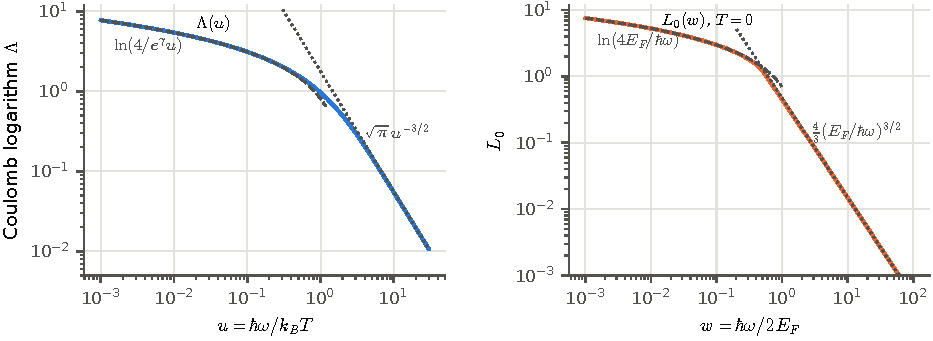
\includegraphics[width=\textwidth]{chapters/pd/fig_lambda.pdf}
\caption{Left, the Coulomb logarithm $\Lambda(u)$ of Maxwell electrons,
Eq.~\eqref{pd:eq:Lambda-mb}, with its asymptotes of
Eq.~\eqref{pd:eq:Lambda-limits}. Right, the function $L_0(w)$ of the degenerate
gas at $T=0$, Eq.~\eqref{pd:eq:nu-T0}, with its asymptotes of
Eq.~\eqref{pd:eq:L0-limits}, against $w=\hbar\omega/2E_F$.}
\label{pd:fig:lambda}
\end{figure}

\subsection{Arbitrary degeneracy}
\label{pd:sec:degenerate}
Insert Eq.~\eqref{pd:eq:imchi-fd} into Eq.~\eqref{pd:eq:nu-weak},
\begin{equation}
\boxed{\;\nueff=\frac{4Ze^4m\kB T}{3\pi\hbar^4\omega}\int_0^\infty\frac{\dd k}{k}\,
\ln\frac{1+e^{(\mu-E_-)/\kB T}}{1+e^{(\mu-E_+)/\kB T}},\qquad
E_\pm=\frac m2\Big(\frac\omega k\pm\frac{\hbar k}{2m}\Big)^2.\;}
\label{pd:eq:nu-fd}
\end{equation}
For $e^{\mu/\kB T}\ll1$ the logarithm is $e^{\mu/\kB T}(e^{-E_-/\kB T}-e^{-E_+/\kB T})$
and Eq.~\eqref{pd:eq:Lambda-mb} follows. The chemical potential is fixed by
$n_e=2\int\dd^3q\,(2\pi\hbar)^{-3}f$. Pauli blocking does not appear, by
Section~\ref{pd:sec:blocking}, but the occupation of the states does.

\subsection{The degenerate electron gas at zero temperature}
{\noindent}(1) At $T=0$, $\kB T\ln[(1+e^{(\mu-E_-)/\kB T})/(1+e^{(\mu-E_+)/\kB T})]
\to(E_F-E_-)_+-(E_F-E_+)_+$, where $(y)_+=\max(y,0)$ and $\mu=E_F=mv_F^2/2$.
With $x=k/k_F$, $k_F=mv_F/\hbar$ and $w=\hbar\omega/2E_F=\omega/k_Fv_F$,
$E_\pm/E_F=(w/x\pm x/2)^2$ and
\begin{equation}
\nueff=\frac{4Ze^4mE_F}{3\pi\hbar^4\omega}\,I_0(w),\qquad
I_0(w)=\int_0^\infty\frac{\dd x}{x}\Big\{\Big[1-\Big(\frac wx-\frac x2\Big)^2\Big]_+
-\Big[1-\Big(\frac wx+\frac x2\Big)^2\Big]_+\Big\}.
\end{equation}

{\noindent}(2) The first bracket is positive for $|w/x-x/2|<1$, that is for
$x_1<x<x_2$ with $x_{1,2}=\sqrt{1+2w}\mp1$. There the integrand is
$(1+w)/x-w^2/x^3-x/4$, with the antiderivative $(1+w)\ln x+w^2/2x^2-x^2/8$.
At the end points $w/x-x/2=\pm1$, and
$\tfrac12(w^2/x^2-x^2/4)=\tfrac12(w/x-x/2)(w/x+x/2)$ equals $(x_1+1)/2$ at $x_1$
and $-(x_2-1)/2$ at $x_2$. Hence
\begin{equation}
I_-(w)=(1+w)\ln\frac{\sqrt{1+2w}+1}{\sqrt{1+2w}-1}-\sqrt{1+2w}.
\end{equation}

{\noindent}(3) The second bracket is positive for $w/x+x/2<1$, which needs
$w<1/2$ and then $x_3<x<x_4$ with $x_{3,4}=1\mp\sqrt{1-2w}$. The same steps,
with the integrand $(1-w)/x-w^2/x^3-x/4$, give
\begin{equation}
I_+(w)=(1-w)\ln\frac{1+\sqrt{1-2w}}{1-\sqrt{1-2w}}-\sqrt{1-2w}\quad(w<\tfrac12),\qquad I_+=0\quad(w\geq\tfrac12).
\end{equation}

{\noindent}(4) With $4Ze^4mE_F/(3\pi\hbar^4\omega)=(4Ze^4m/3\pi\hbar^3)/(2w)$,
\begin{equation}
\boxed{\;\nueff=\frac{4Ze^4m}{3\pi\hbar^3}\,L_0(w),\qquad L_0(w)=\frac{I_-(w)-I_+(w)}{2w},\qquad
w=\frac{\hbar\omega}{2E_F}.\;}
\label{pd:eq:nu-T0}
\end{equation}

{\noindent}(5) For $w\ll1$, $I_-(w)-I_+(w)=2w\ln(2/w)+O(w^2)$, and for
$w\gg1$, $I_-=\tfrac43(2w)^{-1/2}+O(w^{-3/2})$, so
\begin{equation}
\boxed{\;L_0(w)\simeq\ln\frac{4E_F}{\hbar\omega}\quad(\hbar\omega\ll E_F),\qquad
L_0(w)\simeq\frac43\Big(\frac{E_F}{\hbar\omega}\Big)^{3/2}\quad(\hbar\omega\gg E_F).\;}
\label{pd:eq:L0-limits}
\end{equation}
{\noindent}(6) The low-frequency form is the resistivity formula of Ziman.
For an electron at the Fermi surface the Born cross section
$(m/2\pi\hbar^2)^2|\tilde v(q)|^2$ with $q=2k_F\sin(\theta/2)$,
$1-\cos\theta=q^2/2k_F^2$ and $\dd\Omega=2\pi q\,\dd q/k_F^2$ gives the momentum
relaxation rate
\begin{equation}
\frac1\tau=n_iv_F\int(1-\cos\theta)\frac{\dd\sigma}{\dd\Omega}\dd\Omega
=\frac{n_im}{4\pi\hbar^3k_F^3}\int_{k_{\min}}^{2k_F}q^3|\tilde v(q)|^2\,\dd q
=\frac{4Ze^4m}{3\pi\hbar^3}\ln\frac{2k_F}{k_{\min}},
\end{equation}
where the last step uses the Coulomb form and $k_F^3=3\pi^2n_e=3\pi^2Zn_i$.
With the minimum momentum transfer $k_{\min}=\omega/v_F$ that energy
conservation imposes on an electron at the Fermi surface,
$\ln(2k_F/k_{\min})=\ln(4E_F/\hbar\omega)$, and the two agree.

\subsection{The universal high-frequency tail}
{\noindent}(1) When $\hbar\omega$ exceeds every electron energy that is
occupied, Eq.~\eqref{pd:eq:imchi-general} has $E_+=E_-+\hbar\omega$ far above the
occupied energies, and $E_-$ is small only near $k_\omega=(2m\omega/\hbar)^{1/2}$,
where $\omega/k=\hbar k/2m$. There $c_-=\omega/k-\hbar k/2m\simeq-(\hbar/m)(k-k_\omega)$.

{\noindent}(2) Hence
\begin{equation}
\int_0^\infty\frac{\dd k}{k}\int_{E_-}^{E_+}f\,\dd E\simeq\frac{m}{\hbar k_\omega}
\int_{-\infty}^\infty\dd c\int_{mc^2/2}^\infty f(E)\,\dd E
=\frac{m}{\hbar k_\omega}\,2\int_0^\infty f(E)\Big(\frac{2E}{m}\Big)^{1/2}\dd E
=\frac{m}{\hbar k_\omega}\,\frac{n_e(2\pi\hbar)^3}{4\pi m^2},
\end{equation}
where the last step uses $n_e=8\pi m(2\pi\hbar)^{-3}\int(2mE)^{1/2}f\,\dd E$.

{\noindent}(3) With Eq.~\eqref{pd:eq:imchi-general}, $\int_0^\infty\Imag\chi_0\,\dd k=-\pi mn_e/\hbar^2k_\omega$
for every distribution, and Eq.~\eqref{pd:eq:nu-weak} gives
\begin{equation}
\boxed{\;\nueff\;\longrightarrow\;\frac{4\sqrt2\,\pi}{3}\,\frac{Zn_ee^4}{m^{1/2}(\hbar\omega)^{3/2}}.\;}
\label{pd:eq:tail}
\end{equation}
Both the Maxwell form, $\nuT\sqrt\pi u^{-3/2}$, and the degenerate form,
$(4Ze^4m/3\pi\hbar^3)\tfrac43(E_F/\hbar\omega)^{3/2}$ with
$E_F^{3/2}=3\pi^2\hbar^3n_e/(2m)^{3/2}$, reduce to it. When the photon energy
exceeds the kinetic energies the electrons absorb as if they were at rest.

\medskip
\noindent\textbf{Remarks:}\\
(1) For hydrogen at $\kB T=1$~keV and $\lambda_L=0.351~\mu$m,
$u=0.0035$ and $\Lambda=6.45$, while the logarithm of the cutoffs stated
with Eq.~(10.136)~\cite{pd:Atzeni2004} at $n_e=n_c/4$ is $7.58$, and the printed
formula gives $6.69$. The difference between the printed formula and its
stated cutoffs is taken up in Appendix~\ref{pd:app:atzeni-log}.\\
(2) Screening changes the lower limit of the $k$ integral, where $\Imag\chi_0$
is already exponentially small below $k\sim\omega/v_t$. Its effect is computed
in Section~\ref{pd:sec:rpa} and is a few tenths in $\Lambda$ near the critical
density.


\section{Spontaneous bremsstrahlung, the Gaunt factor and Kirchhoff's law}
\label{pd:sec:gaunt}
\subsection{From stimulated to spontaneous emission}
{\noindent}(1) Quantize one mode of the radiation field in the box, with wave
vector $\kv_L$, polarization $\ehat_\lambda$ and frequency $\omega=ck_L$,
\begin{equation}
\hat\Ev=i\Big(\frac{2\pi\hbar\omega}{\Vol}\Big)^{1/2}\ehat_\lambda
\big(\hat a\,e^{i(\kv_L\cdot\rv-\omega t)}-\hat a^\dagger e^{-i(\kv_L\cdot\rv-\omega t)}\big).
\end{equation}
In a state with $N$ photons the absorption matrix element carries
$\langle N-1|\hat a|N\rangle=\sqrt N$ and the emission one
$\langle N+1|\hat a^\dagger|N\rangle=\sqrt{N+1}$.

{\noindent}(2) The classical field $E_0\ehat\cos\omega t$ has the amplitude
$E_0/2$ in front of $e^{-i\omega t}$. For $N\gg1$ it corresponds to
$E_0/2=(2\pi\hbar\omega N/\Vol)^{1/2}$, that is $E_0^2/8\pi=N\hbar\omega/\Vol$, the
energy density of $N$ photons. The weak-field rates of
Section~\ref{pd:sec:onephoton} are therefore $N$ times the rates for one photon,
and the spontaneous emission into the mode is the stimulated rate with
$N\to1$,
\begin{equation}
\boxed{\;W^{\rm sp}_{\pv\to\pv'}(\kv_L,\lambda)=W_{\pv\to\pv'}^{(\ell=-1)}\Big|_{E_0^2=8\pi\hbar\omega/\Vol,\;\ehat=\ehat_\lambda}.\;}
\label{pd:eq:spont-stim}
\end{equation}
This is the content of Einstein's relation, Eqs.~(10.84) and (10.85)~\cite{pd:Atzeni2004}.

\subsection{The Born bremsstrahlung cross section}
{\noindent}(1) With $a_0^2=e^2E_0^2/m^2\omega^4=8\pi\hbar e^2/(\Vol m^2\omega^3)$,
the cross section of Eq.~\eqref{pd:eq:bf} for $\ell=-1$ and one mode is
\begin{equation}
\frac{\dd\sigma}{\dd\Omega'}=\frac{m^2}{4\pi^2\hbar^4}\frac{p'}{p}|\tilde v(\kv)|^2\,
\frac{(\kv\cdot\ehat_\lambda)^2}{4}\,\frac{8\pi\hbar e^2}{\Vol m^2\omega^3}
=\frac{e^2}{2\pi\hbar^3\Vol\omega^3}\,\frac{p'}{p}\,|\tilde v(\kv)|^2(\kv\cdot\ehat_\lambda)^2,
\end{equation}
with $p'=(p^2-2m\hbar\omega)^{1/2}$.

{\noindent}(2) Sum over the modes in vacuum,
$\sum_{\kv_L,\lambda}\to\Vol\sum_\lambda\int\omega^2\dd\omega\,\dd\Omega_L/(2\pi c)^3$.
The two polarizations perpendicular to $\hat\kv_L$ give
$\sum_\lambda(\kv\cdot\ehat_\lambda)^2=k^2-(\kv\cdot\hat\kv_L)^2$, whose integral
over the directions of the photon is $4\pi k^2-\tfrac{4\pi}{3}k^2=\tfrac{8\pi}{3}k^2$.
The emission cross section per unit frequency is
\begin{equation}
\frac{\dd\sigma}{\dd\omega\,\dd\Omega'}=\frac{e^2}{2\pi\hbar^3\omega^3}\,\frac{\omega^2}{8\pi^3c^3}\,
\frac{8\pi}{3}\,\frac{p'}{p}\,k^2|\tilde v(\kv)|^2
=\frac{e^2}{6\pi^3\hbar^3c^3\omega}\,\frac{p'}{p}\,k^2|\tilde v(\kv)|^2.
\label{pd:eq:spont-diff}
\end{equation}

{\noindent}(3) For a Coulomb ion $k^2|\tilde v|^2=16\pi^2Z^2e^4/k^2$, and
$\int\dd\Omega'/k^2=2\pi\hbar^2\int_{-1}^1\dd c/(p^2+p'^2-2pp'c)=(2\pi\hbar^2/pp')L$
with $L=\ln[(p+p')/(p-p')]$, so
\begin{equation}
\boxed{\;\frac{\dd\sigma}{\dd\omega}=\frac{16}{3}\,\frac{Z^2e^6}{m^2c^3\hbar v^2\omega}\,
\ln\frac{p+p'}{p-p'}.\;}
\label{pd:eq:born-brems}
\end{equation}
This is the nonrelativistic Born cross section of bremsstrahlung,
$\dd\sigma=\tfrac{16}{3}Z^2\alpha r_e^2(c^2/v^2)L\,\dd\omega/\omega$ with
$\alpha=e^2/\hbar c$ and $r_e=e^2/mc^2$.

{\noindent}(4) Kramers' cross section of Eq.~\eqref{pd:eq:kramers}, per unit
angular frequency, is $(\dd\sigma/\dd\nu)/2\pi$ with $h\nu=\hbar\omega$, that is
$(16\pi/3\sqrt3)Z^2e^6/(m^2c^3v^2\hbar\omega)$. The ratio is the Born Gaunt factor,
\begin{equation}
\boxed{\;g_B(E,\hbar\omega)=\frac{\sqrt3}{\pi}\ln\frac{p+p'}{p-p'},\qquad
p=(2mE)^{1/2},\quad p'=[2m(E-\hbar\omega)]^{1/2}.\;}
\label{pd:eq:gaunt-born}
\end{equation}
For soft photons $g_B\to(\sqrt3/\pi)\ln(4E/\hbar\omega)$, and at the threshold
$p'\to0$ it vanishes as $(\sqrt3/\pi)2p'/p$.

\subsection{The thermal average}
{\noindent}(1) The emission of a Maxwellian plasma is proportional to
$\int\dd^3v\,f\,v\,\dd\sigma/\dd\omega\propto\int v\,\dd v\,e^{-E/\kB T}g_B
=m^{-1}\int\dd E\,e^{-E/\kB T}g_B$ over $E>\hbar\omega$, while Kramers' form
has $g=1$. The thermally averaged Gaunt factor is therefore
\begin{equation}
\langle g\rangle=\frac{\int_{\hbar\omega}^\infty e^{-E/\kB T}g_B\,\dd E}{\int_{\hbar\omega}^\infty e^{-E/\kB T}\dd E}
=\frac{\sqrt3}{\pi}\,e^u\int_u^\infty e^{-\epsilon}
\ln\frac{\sqrt\epsilon+\sqrt{\epsilon-u}}{\sqrt\epsilon-\sqrt{\epsilon-u}}\,\dd\epsilon,
\end{equation}
with $\epsilon=E/\kB T$.

{\noindent}(2) Substitute $\epsilon=u\cosh^2t$. Then
$\sqrt\epsilon\pm\sqrt{\epsilon-u}=\sqrt u\,e^{\pm t}$, the logarithm is $2t$, and
$\dd\epsilon=u\sinh2t\,\dd t$. With $\cosh^2t=\tfrac12(1+\cosh2t)$ and $\tau=2t$,
\begin{equation}
\int_u^\infty e^{-\epsilon}\ln(\cdots)\,\dd\epsilon
=\frac u2\,e^{-u/2}\int_0^\infty\tau\sinh\tau\,e^{-(u/2)\cosh\tau}\dd\tau.
\end{equation}

{\noindent}(3) Integrate by parts with
$\sinh\tau\,e^{-(u/2)\cosh\tau}=\dd[-(2/u)e^{-(u/2)\cosh\tau}]/\dd\tau$. The
boundary terms vanish, and $\int_0^\infty e^{-z\cosh\tau}\dd\tau=K_0(z)$,
Eq.~(10.32.9)~\cite{pd:DLMF}, leaves $(2/u)K_0(u/2)$. Hence
\begin{equation}
\boxed{\;\langle g\rangle(u)=\frac{\sqrt3}{\pi}\,e^{u/2}K_0\Big(\frac u2\Big).\;}
\label{pd:eq:gaunt-avg}
\end{equation}

{\noindent}(4) The power radiated at all frequencies weights the spectrum
with $e^{-u}$, the factor of Kramers' form, so its Gaunt factor is
\begin{equation}
\boxed{\;\bar g=\int_0^\infty\langle g\rangle(u)\,e^{-u}\,\dd u=\frac{\sqrt3}{\pi}\,2\int_0^\infty e^{-x}K_0(x)\,\dd x
=\frac{2\sqrt3}{\pi}=1.103,\;}
\label{pd:eq:gaunt-power}
\end{equation}
using $K_0(x)=\int_0^\infty e^{-x\cosh t}\dd t$, so that
$\int_0^\infty e^{-x}K_0(x)\dd x=\int_0^\infty\dd t/(1+\cosh t)=[\tanh(t/2)]_0^\infty=1$.
This is the factor $g\approx2\sqrt3/\pi$ that
Atzeni and Meyer-ter-Vehn apply to Eq.~(10.93)~\cite{pd:Atzeni2004}. It is the
Born value exactly.

\subsection{Kirchhoff's law and the Coulomb logarithm as a Gaunt factor}
{\noindent}(1) Compare Eq.~\eqref{pd:eq:gaunt-avg} with Eq.~\eqref{pd:eq:Lambda-mb},
\begin{equation}
\boxed{\;\Lambda(u)=\frac{\pi}{\sqrt3}\,\langle g\rangle(u)\,\frac{1-e^{-u}}{u}.\;}
\label{pd:eq:Lambda-gaunt}
\end{equation}
The quantum Coulomb logarithm of inverse bremsstrahlung is $\pi/\sqrt3$ times
the thermally averaged Gaunt factor, times the stimulated-emission factor
divided by $u$.

{\noindent}(2) The emission coefficient per unit volume, frequency and solid
angle follows from Eq.~\eqref{pd:eq:born-brems} and the steps of the thermal
average,
\begin{equation}
\begin{aligned}
j_\omega&=\frac{n_en_i\hbar\omega}{4\pi}\Big\langle v\,\frac{\dd\sigma}{\dd\omega}\Big\rangle,\qquad
\Big\langle\frac Lv\Big\rangle=\Big(\frac2\pi\Big)^{1/2}\frac{\pi}{\sqrt3}\,\frac{\langle g\rangle e^{-u}}{v_t},\\
j_\omega&=\frac{4}{3\pi}\Big(\frac2\pi\Big)^{1/2}\frac{n_en_iZ^2e^6}{m^2c^3v_t}\,\frac{\pi}{\sqrt3}\langle g\rangle e^{-u}.
\end{aligned}
\end{equation}
The absorption coefficient of Eq.~\eqref{pd:eq:drude-K} with $n_r=1$ and
$\nueff=\nuT\Lambda$, multiplied by the Planck function per unit angular
frequency and solid angle, $B_\omega=(\hbar\omega^3/4\pi^3c^2)/(e^u-1)$, is, by
Eq.~\eqref{pd:eq:Lambda-gaunt},
\begin{equation}
K\,B_\omega=\frac{\nuT\omega_p^2}{c\omega^2}\,\frac{\pi}{\sqrt3}\langle g\rangle\frac{e^{-u}}{u}\,\frac{\hbar\omega^3}{4\pi^3c^2}
=\frac{4\sqrt{2\pi}}{3\pi^2}\,\frac{n_en_iZ^2e^6}{m^{3/2}(\kB T)^{1/2}c^3}\,\frac{\pi}{\sqrt3}\langle g\rangle e^{-u}.
\end{equation}
Since $m^2v_t=m^{3/2}(\kB T)^{1/2}$ and $\tfrac{4}{3\pi}(2/\pi)^{1/2}=\tfrac{4\sqrt{2\pi}}{3\pi^2}$,
\begin{equation}
\boxed{\;j_\omega=K\,B_\omega.\;}
\label{pd:eq:kirchhoff}
\end{equation}
Kirchhoff's law holds exactly between the absorption of the master equation
and the spontaneous emission of Eq.~\eqref{pd:eq:born-brems}, because both come
from the same matrix element and the Maxwellian satisfies detailed balance.

\medskip
\noindent\textbf{In Summary:} The free--free emission and the inverse
bremsstrahlung absorption of the quantum theory are Kramers' expressions
multiplied by the Born Gaunt factor. Its thermal average is
$(\sqrt3/\pi)e^{u/2}K_0(u/2)$, its power average is $2\sqrt3/\pi$, and the
Coulomb logarithm of the absorption is the Gaunt factor in disguise,
Eq.~\eqref{pd:eq:Lambda-gaunt}.

\section{The interacting electron gas and dynamic screening}
\label{pd:sec:manybody}
\subsection{The oscillating frame for many electrons}
{\noindent}(1) The Hamiltonian of $N$ electrons in the laser field and the
field of the ions is
\begin{equation}
H=\sum_{a=1}^N\frac{1}{2m}\Big[\hat\pv_a+\frac ec\Av(t)\Big]^2
+\sum_{a<b}\frac{e^2}{|\hat\rv_a-\hat\rv_b|}+\sum_aV(\hat\rv_a),
\end{equation}
apart from the constant energy of the fixed ions.

{\noindent}(2) Let $\hat T=\exp[-(i/\hbar)\boldsymbol\alpha(t)\cdot\hat{\mathbf P}]$
with $\hat{\mathbf P}=\sum_a\hat\pv_a$. It translates all electrons together, so
the electron--electron interaction, which depends on differences, is
unchanged, $\hat T^\dagger V_{ee}\hat T=V_{ee}$. The steps of
Section~\ref{pd:sec:KH1}, with $\dot S=Ne^2A^2/2mc^2$, give
\begin{equation}
\boxed{\;H'=\sum_a\frac{\hat p_a^2}{2m}+\sum_{a<b}\frac{e^2}{|\hat\rv_a-\hat\rv_b|}
+\sum_aV\big(\hat\rv_a+\boldsymbol\alpha(t)\big).\;}
\label{pd:eq:H-KH}
\end{equation}
In the oscillating frame the electron gas carries no field, and the ions are
external charges that move along $\Rv_j-\boldsymbol\alpha(t)$. A uniform field
couples only to the center of mass of the electrons \cite{pd:Kohn1961}, which is
the content of this transformation.

\subsection{The absorbed power in the two frames}
{\noindent}(1) The power that the laser delivers to the electrons in the
laboratory is $P_{\rm lab}(t)=-e\Ev(t)\cdot\sum_a\langle\vv_a\rangle$, with the
velocity $\vv_a=(\hat\pv_a+e\Av/c)/m$. Since $\hat T$ commutes with
$\hat\pv_a$, $\sum_a\langle\vv_a\rangle=\langle\hat{\mathbf P}\rangle'/m+N\dot{\boldsymbol\alpha}$,
where the prime marks an average in the oscillating frame. The term
$-eN\Ev\cdot\dot{\boldsymbol\alpha}\propto\cos\omega t\sin\omega t$ averages to
zero over a period.

{\noindent}(2) In the oscillating frame,
$\dd\langle H'\rangle/\dd t=\langle\partial_tH'\rangle=-\dot{\boldsymbol\alpha}\cdot\langle\mathbf F\rangle'$,
with the force $\mathbf F=-\sum_a\nabla V(\hat\rv_a+\boldsymbol\alpha)$ of the ions
on the electrons. The total momentum obeys
$\dd\langle\hat{\mathbf P}\rangle'/\dd t=\langle\mathbf F\rangle'$, because the
kinetic term commutes with $\hat{\mathbf P}$ and the internal forces cancel.
With $\ddot{\boldsymbol\alpha}=-e\Ev/m$,
\begin{equation}
\frac{\dd\langle H'\rangle}{\dd t}=-\dot{\boldsymbol\alpha}\cdot\frac{\dd\langle\hat{\mathbf P}\rangle'}{\dd t}
=-\frac{\dd}{\dd t}\big(\dot{\boldsymbol\alpha}\cdot\langle\hat{\mathbf P}\rangle'\big)
-\frac em\Ev\cdot\langle\hat{\mathbf P}\rangle'.
\end{equation}

{\noindent}(3) In the steady state $\langle\hat{\mathbf P}\rangle'$ is
periodic, and the total derivative averages to zero. Hence
\begin{equation}
\boxed{\;\langle P_{\rm lab}\rangle_t=\Big\langle\frac{\dd\langle H'\rangle}{\dd t}\Big\rangle_t.\;}
\label{pd:eq:frames}
\end{equation}
The absorbed power is the rate at which the energy of the electron gas grows
in the oscillating frame.

\subsection{Linear response to the oscillating ions}
{\noindent}(1) With the density operator $\hat n_{\kv}=\sum_ae^{-i\kv\cdot\hat\rv_a}$
and Eq.~\eqref{pd:eq:Vk}, the ion term of Eq.~\eqref{pd:eq:H-KH} is
\begin{equation}
\sum_aV(\hat\rv_a+\boldsymbol\alpha)=\frac1\Vol\sum_{\kv}U_{\kv}(t)\,\hat n_{-\kv},\qquad
U_{\kv}(t)=\tilde V(\kv)\,e^{i\kv\cdot\boldsymbol\alpha(t)}
=\tilde V(\kv)\sum_\ell i^\ell J_\ell(\kv\cdot\av)\,e^{i\ell\omega t},
\label{pd:eq:Uk}
\end{equation}
by Eq.~\eqref{pd:eq:jacobi-anger}. In this frame the ion potential is a sum of
harmonics $\ell\omega$ with the weights $J_\ell$.

{\noindent}(2) Let the electron gas start in equilibrium. To first order in
$U$, Kubo's formula gives
$\delta\langle\hat n_{\kv}\rangle'(t)=\int\chi(\kv,t-t')U_{\kv}(t')\dd t'$ with
the retarded density response
\begin{equation}
\chi(\kv,t)=-\frac i\hbar\,\theta(t)\,\frac1\Vol\big\langle[\hat n_{\kv}(t),\hat n_{-\kv}(0)]\big\rangle,\qquad
\chi(\kv,\Omega)=\int e^{i\Omega t}\chi(\kv,t)\,\dd t,
\end{equation}
which for free electrons is the Lindhard function of Eq.~\eqref{pd:eq:chi0}
\cite{pd:GiulianiVignale2005}. A harmonic $e^{i\ell\omega t}=e^{-i(-\ell\omega)t}$
is answered with the factor $\chi(\kv,-\ell\omega)$.

{\noindent}(3) The power in the oscillating frame is
$\dd\langle H'\rangle/\dd t=\Vol^{-1}\sum_{\kv}\partial_tU_{\kv}\,\langle\hat n_{-\kv}\rangle'$.
The term $\kv=0$ is constant. With
$U_{-\kv}=\tilde V(-\kv)\sum_\ell(-i)^\ell J_\ell(\kv\cdot\av)e^{i\ell\omega t}$, the
response $\delta\langle\hat n_{-\kv}\rangle'=\sum_\ell\chi(-\kv,-\ell\omega)U_{-\kv,\ell}e^{i\ell\omega t}$,
and $\partial_tU_{\kv}=\sum_{\ell'}i\ell'\omega U_{\kv,\ell'}e^{i\ell'\omega t}$, the
period average keeps $\ell'=-\ell$. The product of the coefficients is
$\tilde V(\kv)\tilde V(-\kv)\,i^{-\ell}J_{-\ell}(-i)^\ell J_\ell=|\tilde V(\kv)|^2J_\ell^2$,
and with $\chi(-\kv,-\Omega)=\chi(\kv,\Omega)^*$,
\begin{equation}
\Big\langle\frac{\dd\langle H'\rangle}{\dd t}\Big\rangle_t
=\frac1\Vol\sum_{\kv}\sum_\ell(-i\ell\omega)|\tilde V(\kv)|^2J_\ell^2\,\chi(\kv,\ell\omega)^*
=-\frac1\Vol\sum_{\kv}\sum_\ell\ell\omega\,|\tilde V(\kv)|^2J_\ell^2\,\Imag\chi(\kv,\ell\omega),
\end{equation}
where the terms with $\Real\chi$, which is even in the frequency for the
isotropic gas, cancel between $\ell$ and $-\ell$.

{\noindent}(4) After the average over the ion positions and per unit
volume, by Eq.~\eqref{pd:eq:frames},
\begin{equation}
\boxed{\;P=-n_i\sum_{\ell=-\infty}^\infty\ell\omega\int\frac{\dd^3k}{(2\pi)^3}\,|\tilde v(\kv)|^2S(\kv)\,
J_\ell^2(\kv\cdot\av)\,\Imag\chi(\kv,\ell\omega).\;}
\label{pd:eq:P-KH}
\end{equation}
This is Eq.~\eqref{pd:eq:P-chi0} with $\chi_0$ replaced by the density response
of the interacting gas. For free electrons the two derivations agree term by
term, because the Volkov states of the laboratory are the plane waves of the
oscillating frame. The result is exact to second order in the ion potential
and exact in the field.

\subsection{The dielectric form}
{\noindent}(1) The longitudinal dielectric function is defined by
$1/\varepsilon(\kv,\Omega)=1+v_c(k)\chi(\kv,\Omega)$ with $v_c=4\pi e^2/k^2$.
In the random-phase approximation $\varepsilon=1-v_c\chi_0$ and $\chi=\chi_0/\varepsilon$.
For a Coulomb ion,
$|\tilde v|^2\Imag\chi=(4\pi Ze^2/k^2)^2(k^2/4\pi e^2)\Imag\varepsilon^{-1}=(4\pi Z^2e^2/k^2)\Imag\varepsilon^{-1}$,
and
\begin{equation}
\boxed{\;P=-n_iZ^2e^2\sum_{\ell=-\infty}^\infty\ell\omega\int\frac{\dd^3k}{(2\pi)^3}\,\frac{4\pi}{k^2}\,S(\kv)\,
J_\ell^2(\kv\cdot\av)\,\Imag\frac{1}{\varepsilon(\kv,\ell\omega)}.\;}
\label{pd:eq:P-silin}
\end{equation}
With the classical dielectric function this is Silin's result \cite{pd:Silin1965}.
With the Lindhard dielectric function it is the quantum form obtained by Kull
and Plagne \cite{pd:KullPlagne2001} and by Bornath and co-workers
\cite{pd:Bornath2001} from the quantum Vlasov and the quantum kinetic equation.

{\noindent}(2) For weak fields Eq.~\eqref{pd:eq:nu-weak} with
$k^4|\tilde v|^2\Imag\chi=4\pi Z^2e^2k^2\Imag\varepsilon^{-1}$ gives
\begin{equation}
\boxed{\;\nueff(\omega)=-\frac{2Ze^2}{3\pi m\omega}\int_0^\infty k^2S(k)\,\Imag\frac{1}{\varepsilon(k,\omega)}\,\dd k,\;}
\label{pd:eq:dawson-oberman}
\end{equation}
the high-frequency collision frequency of Dawson and Oberman
\cite{pd:DawsonOberman1962}.

\subsection{Dynamic screening for Maxwell electrons}
\label{pd:sec:rpa}
{\noindent}(1) For nondegenerate electrons the Lindhard function follows from
Eq.~\eqref{pd:eq:chi0} with the shift $\mathbf q\to\mathbf q-\hbar\kv$ in its
second term and the integral over $\mathbf q_\perp$, which leaves the
one-dimensional Maxwellian $g_1(v)=(2\pi v_t^2)^{-1/2}e^{-v^2/2v_t^2}$,
\begin{equation}
\chi_0=\frac{n_e}{\hbar k}\int g_1(v)\Big[\frac{1}{c_--v+i0^+}-\frac{1}{c_+-v+i0^+}\Big]\dd v
=\frac{n_e}{\sqrt2\,\hbar kv_t}\big[Z(\zeta_+)-Z(\zeta_-)\big],\qquad
\zeta_\pm=\frac{c_\pm}{\sqrt2v_t},
\label{pd:eq:chi0-Z}
\end{equation}
with $c_\pm=\Omega/k\pm\hbar k/2m$ and the plasma dispersion function
$Z(\zeta)=\pi^{-1/2}\int e^{-t^2}(t-\zeta)^{-1}\dd t$ for $\Imag\zeta>0$
\cite{pd:FriedConte1961}. Its imaginary part on the real axis is
$\sqrt\pi e^{-\zeta^2}$, which gives back Eq.~\eqref{pd:eq:imchi-mb}.

{\noindent}(2) In the classical limit $Z(\zeta_+)-Z(\zeta_-)\to(\hbar k/\sqrt2mv_t)Z'(\zeta)$
with $Z'=-2(1+\zeta Z)$, so $\chi_0\to-(n_e/\kB T)[1+\zeta Z(\zeta)]$ and
$\varepsilon=1+(k_D^2/k^2)[1+\zeta Z(\zeta)]$ with $k_D^2=4\pi e^2n_e/\kB T$. This is
Eq.~(11.19)~\cite{pd:Atzeni2004}, whose function $W$ is $W(x)=1+(x/\sqrt2)Z(x/\sqrt2)$.

{\noindent}(3) With $x=kv_t/\omega$, $r=\omega_p/\omega$, $\hbar kv_t/\kB T=ux$ and
$k_D^2/k^2=r^2/x^2$,
\begin{equation}
\varepsilon(x)=1-\frac{r^2}{\sqrt2\,ux^3}\big[Z(\zeta_+)-Z(\zeta_-)\big],\qquad
\zeta_\pm=\frac{1}{\sqrt2}\Big(\frac1x\pm\frac{ux}{2}\Big).
\end{equation}
Equation~\eqref{pd:eq:dawson-oberman} with $S=1$, divided by $\nuT$, becomes
\begin{equation}
\boxed{\;\nueff=\nuT\Lambda_{\rm RPA}(r,u),\qquad
\Lambda_{\rm RPA}(r,u)=-\frac{1}{r^2}\Big(\frac2\pi\Big)^{1/2}\int_0^\infty x^2\,\Imag\frac{1}{\varepsilon(x)}\,\dd x.\;}
\label{pd:eq:Lambda-rpa}
\end{equation}
Without screening $\Imag\varepsilon^{-1}\to-\Imag\varepsilon$, the integral
becomes $u^{-1}\int x^{-1}[e^{-\zeta_-^2}-e^{-\zeta_+^2}]\dd x$, and
Eq.~\eqref{pd:eq:Lambda-mb} returns.

{\noindent}(4) Table~\ref{pd:tab:rpa} and Fig.~\ref{pd:fig:rpa} give the screening correction. It is
negative and nearly independent of $u$. It is $-0.10$ at $n_e=n_c/4$ and $-0.47$ at
$n_e=0.94\,n_c$, and it approaches $-0.56$ as $\omega\to\omega_p$ for $u\ll1$, slowly,
because the resonance described next carries a weight proportional to
$(1-r^2)^{1/2}$. For $\omega>\omega_p$ the function $\Real\varepsilon$ vanishes
at the Langmuir wave number, approximately $x_{\rm pl}^2=(r^{-2}-1)/3$, where
the ion oscillation excites plasma waves. That resonance is part of the
integral. Its weight, estimated with the Bohm--Gross form
$\Real\varepsilon\simeq1-r^2(1+3x^2)$, is $\sqrt{2\pi}\,x_{\rm pl}/6r^4$, of order
$0.1$ for $r\geq0.9$. For smaller $r$ the plasma waves at $x_{\rm pl}$ are
strongly Landau damped and there is no separate resonance.

\begin{table}[ht]
\centering
\caption{The screening correction $\Lambda_{\rm RPA}-\Lambda$ of the Coulomb
logarithm, Eqs.~\eqref{pd:eq:Lambda-rpa} and \eqref{pd:eq:Lambda-mb}, against
$r=\omega_p/\omega=(n_e/n_c)^{1/2}$.}
\label{pd:tab:rpa}
\begin{tabular}{cccccccc}
\toprule
$u$ & $r=0.95$ & $0.9$ & $0.8$ & $0.7$ & $0.5$ & $0.3$ & $0.1$\\
\midrule
0.003 & $-0.440$ & $-0.375$ & $-0.278$ & $-0.204$ & $-0.099$ & $-0.034$ & $-0.004$\\
0.03  & $-0.439$ & $-0.374$ & $-0.277$ & $-0.203$ & $-0.098$ & $-0.034$ & $-0.004$\\
0.3   & $-0.393$ & $-0.333$ & $-0.244$ & $-0.178$ & $-0.085$ & $-0.029$ & $-0.003$\\
\bottomrule
\end{tabular}
\end{table}

\begin{figure}[ht]
\centering
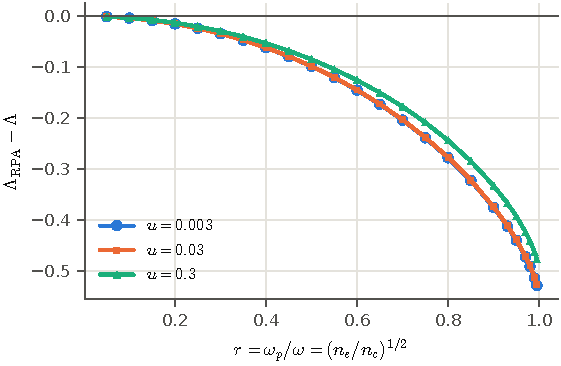
\includegraphics[width=0.62\textwidth]{chapters/pd/fig_rpa.pdf}
\caption{The screening correction $\Lambda_{\rm RPA}-\Lambda$ of
Table~\ref{pd:tab:rpa} against $r=\omega_p/\omega$ for three photon energies.}
\label{pd:fig:rpa}
\end{figure}

\medskip
\noindent\textbf{Remarks:}\\
(1) Without ions $H'$ does not depend on time and nothing is absorbed.
Collisions between electrons alone do not absorb light in the dipole
approximation. They enter only through $\chi$, by screening, and through the
shape of $f$.\\
(2) Equation~\eqref{pd:eq:P-KH} holds for any response function. Local-field
corrections and strong coupling enter through $\chi$, and correlated ions
through $S(k)$.\\
(3) The same result follows from the Kadanoff--Baym equations with the
dynamically screened Born self-energy \cite{pd:Kremp1999,pd:Bornath2001}, which is the
many-body counterpart of the nonequilibrium Green-function route of
Section~3 of the quantum Boltzmann equation paper \cite{pd:Watson2026}.


\section{Strong fields}
\label{pd:sec:strong}
\subsection{The exact heating rate for Maxwell electrons}
{\noindent}(1) Take Eq.~\eqref{pd:eq:P-chi0} with bare Coulomb ions, $S=1$ and an
isotropic distribution. At fixed $k$ the direction of $\kv$ enters only through
$\mu=\hat\kv\cdot\ehat$, and $\int\dd\Omega_kJ_\ell^2(ka_0\mu)=2\pi B_\ell(ka_0)$
with
\begin{equation}
B_\ell(z)=\int_{-1}^1J_\ell^2(z\mu)\,\dd\mu=\frac2z\int_0^zJ_\ell^2(t)\,\dd t.
\end{equation}
With $|\tilde v|^2=16\pi^2Z^2e^4/k^4$,
\begin{equation}
P=-4n_iZ^2e^4\sum_\ell\ell\omega\int_0^\infty\frac{\dd k}{k^2}\,\Imag\chi_0(k,\ell\omega)\,B_\ell(ka_0).
\end{equation}

{\noindent}(2) With $x=kv_t/\omega$ and $\beta=v_0/v_t$, $ka_0=x\beta$, and
Eq.~\eqref{pd:eq:imchi-mb} at $\Omega=\ell\omega$ has
$E_\pm/\kB T=\tfrac12(\ell/x\pm ux/2)^2$ and $\hbar kv_t=ux\,\kB T$. Dividing by
$n_emv_0^2/2$ and by $\nuT$,
\begin{equation}
\boxed{\;\begin{aligned}
\nueff&=\nuT\,\frac{3\,\mathcal S(\beta,u)}{u\beta^2},\qquad
\mathcal S(\beta,u)=\sum_{\ell=-\infty}^\infty\ell\int_0^\infty\frac{\dd x}{x^3}\,D_\ell(x)\,B_\ell(x\beta),\\
D_\ell(x)&=e^{-\frac12(\frac\ell x-\frac{ux}2)^2}-e^{-\frac12(\frac\ell x+\frac{ux}2)^2}.
\end{aligned}\;}
\label{pd:eq:S-exact}
\end{equation}
The terms $\pm\ell$ are equal. For $\beta\to0$, $B_{\pm1}\to(x\beta)^2/6$, and
Eq.~\eqref{pd:eq:K0-integral} gives the weak-field limit on the left below,
which is Eq.~\eqref{pd:eq:Lambda-mb}. The nonlinearity is measured by the ratio
on the right,
\begin{equation}
\mathcal S\;\xrightarrow{\;\beta\to0\;}\;\frac{\beta^2}{3}\,2\sinh\frac u2\,K_0\Big(\frac u2\Big),\qquad
R(\beta,u)=\frac{\nueff(v_0)}{\nueff(0)}=\frac{3\,\mathcal S(\beta,u)}{u\beta^2\Lambda(u)}.
\end{equation}

{\noindent}(3) The functions $B_\ell$ follow from a recursion. The recurrences
of the Bessel functions, Eq.~(10.6.2)~\cite{pd:DLMF}, give
$\dd[z(J_\ell^2+J_{\ell+1}^2)]/\dd z=(2\ell+1)(J_\ell^2-J_{\ell+1}^2)$, so
\begin{equation}
\int_0^zJ_\ell^2\,\dd t=\int_0^zJ_{\ell+1}^2\,\dd t+\frac{z\,[J_\ell^2(z)+J_{\ell+1}^2(z)]}{2\ell+1},
\label{pd:eq:Bl-recursion}
\end{equation}
which is summed downward from an order $\ell\gg z$ at which the integral
vanishes. The terms added are positive, and the recursion is stable.

\subsection{The quasi-static limit}
{\noindent}(1) For $x\gg1$, that is $k\gg\omega/v_t$, the function
$\ell\mapsto\ell D_\ell(x)$ changes on the scale $\Delta\ell\sim x$, much larger than
one, and the limit of Eq.~\eqref{pd:eq:arcsine} applies to the sum over $\ell$ at
fixed $k$,
\begin{equation}
\sum_\ell\ell\,D_\ell(x)\,J_\ell^2(x\beta\mu)\;\longrightarrow\;
\frac{1}{2\pi}\int_0^{2\pi}\nu\,D_\nu(x)\,\dd\theta,\qquad \nu=x\beta\mu\cos\theta.
\end{equation}

{\noindent}(2) In dimensional form the frequency $\ell\omega$ becomes the
instantaneous Doppler frequency $\Omega_t=\kv\cdot\vosc(t)$, up to a sign that
does not matter because $\Omega\Imag\chi_0(k,\Omega)$ is even in $\Omega$,
\begin{equation}
\boxed{\;P\;\longrightarrow\;-n_i\int\frac{\dd^3k}{(2\pi)^3}\,|\tilde v(\kv)|^2S(\kv)\,
\big\langle\Omega_t\Imag\chi_0(\kv,\Omega_t)\big\rangle_t,\qquad\Omega_t=\kv\cdot\vosc(t).\;}
\label{pd:eq:quasi-static}
\end{equation}
The ions move through the electron gas of the oscillating frame with the
velocity $-\vosc(t)$, and Eq.~\eqref{pd:eq:quasi-static} is the stopping power of
the dielectric theory of Section~11.5 of \cite{pd:Atzeni2004} at that velocity,
times the velocity, averaged over the period. This is Silin's picture.

{\noindent}(3) The limit fails for $k\lesssim\omega/v_t$. There every term of the
exact sum carries $e^{-\ell^2/2x^2}\leq e^{-1/2x^2}$ and is exponentially small,
even when $v_0\gg v_t$, because the electron gas of the oscillating frame is
thermal and the ions supply only the frequencies $\ell\omega$. The exact sum
therefore keeps the lower cutoff $k\sim\omega/v_t$ at all field strengths, while
the quasi-static formula needs it put in.

\subsection{The classical evaluation and Silin's formula}
{\noindent}(1) In the classical limit, Eq.~\eqref{pd:eq:imchi-classical} with
$\zeta=\Omega_t/\sqrt2kv_t=s\mu$, where $s=s_0\cos\theta$ and
$s_0=v_0/\sqrt2v_t$, gives
$\Omega_t\Imag\chi_0=-(n_e/\kB T)\sqrt\pi\,\sqrt2kv_t\,\zeta^2e^{-\zeta^2}$. The
integrand of Eq.~\eqref{pd:eq:quasi-static} is then $k^{-3}$ times a function of
direction, and the logarithmic integral $\int\dd k/k$ between the two cutoffs
is the Coulomb logarithm, held fixed here.

{\noindent}(2) The angular integral is
\begin{equation}
\int\dd\Omega_k\,\zeta^2e^{-\zeta^2}=2\pi\int_{-1}^1s^2\mu^2e^{-s^2\mu^2}\dd\mu=\pi g(s),\qquad
g(s)=4s^2\int_0^1\tau^2e^{-s^2\tau^2}\dd\tau=\frac{\sqrt\pi\erf s}{s}-2e^{-s^2},
\label{pd:eq:g-function}
\end{equation}
where the last form follows by one integration by parts. For small $s$,
$g=\tfrac43s^2-\tfrac45s^4+\tfrac27s^6+O(s^8)$.

{\noindent}(3) At fixed logarithm the heating rate is proportional to
$\langle g(s_0\cos\theta)\rangle_\theta$, and its weak-field value is
$\tfrac43s_0^2\langle\cos^2\theta\rangle=\tfrac23s_0^2$. The ratio of the strong-field
collision frequency to the weak-field one is therefore
\begin{equation}
\boxed{\;G(s_0)=\frac{3\,\langle g(s_0\cos\theta)\rangle_\theta}{2s_0^2},\qquad s_0=\frac{v_0}{\sqrt2\,v_t}.\;}
\label{pd:eq:G}
\end{equation}

{\noindent}(4) Silin's form follows from the integral representation of $g$.
With $\langle e^{-a\cos^2\theta}\rangle=e^{-a/2}I_0(a/2)$, from
Eq.~(10.32.1)~\cite{pd:DLMF}, and $I_0'=I_1$, Eq.~(10.29.3)~\cite{pd:DLMF},
\begin{equation}
\big\langle\cos^2\theta\,e^{-a\cos^2\theta}\big\rangle=-\frac{\dd}{\dd a}\Big[e^{-a/2}I_0\Big(\frac a2\Big)\Big]
=\frac12e^{-a/2}\Big[I_0\Big(\frac a2\Big)-I_1\Big(\frac a2\Big)\Big].
\end{equation}
With $a=s_0^2\tau^2$ and $z=s_0\tau/\sqrt2$,
\begin{equation}
\begin{aligned}
\langle g(s_0\cos\theta)\rangle&=4s_0^2\int_0^1\tau^2\big\langle\cos^2\theta\,e^{-s_0^2\tau^2\cos^2\theta}\big\rangle\dd\tau
=\frac{4\sqrt2}{s_0}\,Q(r),\\
Q(r)&=\int_0^rz^2e^{-z^2}\big[I_0(z^2)-I_1(z^2)\big]\dd z,
\end{aligned}
\end{equation}
with $r=s_0/\sqrt2=v_0/2v_t$. Since $s_0^3=2\sqrt2r^3$,
\begin{equation}
\boxed{\;G=\frac{3\,Q(r)}{r^3},\qquad r=\frac{v_0}{2v_t}=\frac{eE_0}{2m\omega v_t},\;}
\label{pd:eq:silin-Q}
\end{equation}
which is Eqs.~(3.10) and (3.11)~\cite{pd:Silin1965}. Silin writes
\begin{equation}
\nu=\frac{32\sqrt{2\pi}N_ie_i^2e^2}{m^2v_T^3}\Big(\frac{m\omega v_T}{eE_0}\Big)^3Q(r)\ln\frac{k_{\max}}{k_{\min}}
\end{equation}
with $e_i=Ze$ and $N_i=n_i$. Since $m\omega v_T/eE_0=v_t/v_0=1/2r$ and
$32\sqrt{2\pi}/8r^3=\tfrac43\sqrt{2\pi}\cdot3/r^3$, his $\nu$ is
$\nuT\ln(k_{\max}/k_{\min})\cdot3Q(r)/r^3$.

{\noindent}(5) The limits. For small $s_0$, with
$\langle\cos^{2n}\theta\rangle=(2n-1)!!/(2n)!!$, the series of $g$ gives
$\langle g\rangle=\tfrac23s_0^2-\tfrac{3}{10}s_0^4+\tfrac{5}{56}s_0^6$. For large
$s_0$ write $\langle g(s_0\cos\theta)\rangle=(2/\pi)\int_0^{s_0}g(s)(s_0^2-s^2)^{-1/2}\dd s$
and split $g$ into $\sqrt\pi\erf(s)/s$ and $-2e^{-s^2}$. With
$\int_0^S\erf(s)/s\,\dd s=\ln S+\gamma/2+\ln2+o(1)$,
$\int_0^1[(1-x^2)^{-1/2}-1]\dd x/x=\ln2$ and $\int_0^\infty2e^{-s^2}\dd s=\sqrt\pi$,
proved in Appendix~\ref{pd:app:math},
\begin{equation}
\langle g(s_0\cos\theta)\rangle=\frac{2}{\sqrt\pi\,s_0}\Big[\ln(4s_0)+\frac\gamma2-1\Big]+o(s_0^{-1}).
\end{equation}
Hence
\begin{equation}
\boxed{\;\begin{aligned}
&G=1-\frac{9}{20}s_0^2+\frac{15}{112}s_0^4+O(s_0^6)\quad(s_0\ll1),\qquad
G\simeq\frac{3}{\sqrt\pi s_0^3}\Big[\ln(4s_0)+\frac\gamma2-1\Big]\quad(s_0\gg1),\\
&Q(r)\simeq\frac{\ln r+c_S}{2\sqrt{2\pi}},\qquad c_S=\ln(4\sqrt2)+\frac\gamma2-1=1.0215.
\end{aligned}\;}
\label{pd:eq:G-limits}
\end{equation}
Silin found $Q(r)\simeq(\ln r+1)/2\sqrt{2\pi}$, the $1$ being, in his words,
the result of numerical integration \cite[Eq.~(3.13)]{pd:Silin1965}. The
constant is $c_S=\ln(4\sqrt2)+\gamma/2-1$.

\subsection{The quantum strong-field result}
{\noindent}(1) Table~\ref{pd:tab:strong} compares the exact ratio
$R(\beta,u)$ of Eq.~\eqref{pd:eq:S-exact} with Silin's $G(\beta/\sqrt2)$ at $u=0.3$.
The two agree for weak fields and part for strong ones, where the quantum
result is larger by a factor that grows slowly with $\beta$.

{\noindent}(2) The reason is the upper cutoff. In the quantum theory the
momentum transfer is limited by backscattering of an electron from the moving
ion, $\hbar k\lesssim2m|\hat\kv\cdot\vosc(t)|$, which grows with the field, while the
lower cutoff stays at $k\sim\omega/v_t$ by step~(3) of the quasi-static limit.
At fixed logarithm both cutoffs are held. Figure~\ref{pd:fig:strong} shows the
ratio for three photon energies.

\begin{table}[ht]
\centering
\caption{The ratio $R=\nueff(v_0)/\nueff(0)$ of the exact quantum heating rate,
Eq.~\eqref{pd:eq:S-exact} at $u=0.3$, and Silin's ratio at fixed logarithm,
Eq.~\eqref{pd:eq:silin-Q}, against $\beta=v_0/v_t$.}
\label{pd:tab:strong}
\begin{tabular}{ccccccc}
\toprule
$\beta$ & 0.05 & 0.25 & 1 & 2 & 4 & 8\\
\midrule
$R(\beta,0.3)$ & 0.9996 & 0.9909 & 0.8673 & 0.5909 & 0.2102 & 0.0440\\
$G(\beta/\sqrt2)$ & 0.9994 & 0.9861 & 0.8050 & 0.4604 & 0.1242 & 0.0224\\
\bottomrule
\end{tabular}
\end{table}

\begin{figure}[ht]
\centering
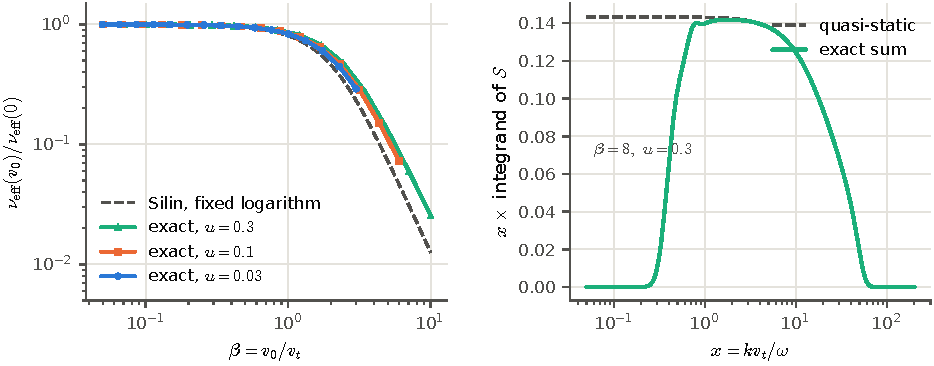
\includegraphics[width=\textwidth]{chapters/pd/fig_strong.pdf}
\caption{Strong fields. Left, the ratio $R=\nueff(v_0)/\nueff(0)$ of the exact
quantum heating rate of Eq.~\eqref{pd:eq:S-exact} for three photon energies,
and Silin's ratio $G$ at fixed logarithm, Eq.~\eqref{pd:eq:silin-Q}. Right, the
integrand of $\mathcal S$ times $x=kv_t/\omega$ at $\beta=8$, $u=0.3$, exact and in
the quasi-static limit of Eq.~\eqref{pd:eq:quasi-static}. The exact integrand is
cut off near $x\approx0.3$ by the thermal factor, and both are cut off near
$x\approx2\beta/u$ by the quantum limit on the momentum transfer.}
\label{pd:fig:strong}
\end{figure}


\section{The kinetic equation of an isotropic distribution}
\label{pd:sec:langdon}
This section returns to the master equation and follows the distribution of
the electrons, not only its energy. Let $F(v)$ be the isotropic velocity
distribution, $n_e=\int4\pi v^2F\,\dd v$, which is $2m^3f/(2\pi\hbar)^3$ in
terms of the occupation numbers.

\subsection{The averaged master equation for weak fields}
{\noindent}(1) For weak fields the master equation~\eqref{pd:eq:master} has the
terms $\ell=0,\pm1$. The term $\ell=0$ connects states of equal energy and
vanishes for an isotropic distribution. The field generates an anisotropy
proportional to $(\hat\pv\cdot\ehat)^2-\tfrac13$, which elastic collisions remove
faster than the field heats, and the isotropic part obeys the master equation
averaged over the direction of $\pv$,
\begin{equation}
\frac{\partial F(E)}{\partial t}=R_+(E)\big[F(E+\hbar\omega)-F(E)\big]+R_-(E)\big[F(E-\hbar\omega)-F(E)\big],
\end{equation}
where $R_\pm=n_iv\bar\sigma_{\pm1}$ with the cross sections of
Eq.~\eqref{pd:eq:sigma-iso},
\begin{equation}
\boxed{\;R_\pm(E)=\frac{2\pi}{3}\,\frac{n_iZ^2e^4a_0^2m}{\hbar^2p}\,L_\pm,\qquad
L_\pm=\ln\frac{p+p'_\pm}{|p-p'_\pm|},\qquad R_-(E)=0\;\;\text{for}\;\;E<\hbar\omega.\;}
\label{pd:eq:Rpm}
\end{equation}

{\noindent}(2) The density of states per unit energy and volume is
$g(E)=2\cdot4\pi p^2(2\pi\hbar)^{-3}\dd p/\dd E=8\pi mp/(2\pi\hbar)^3$, so
$g(E)R_+(E)$ is proportional to $L_+(p)$, which is symmetric in $p$ and
$p'_+$. Since $L_-$ at the momentum $p'_+$ is the same logarithm,
\begin{equation}
\boxed{\;g(E)\,R_+(E)=g(E+\hbar\omega)\,R_-(E+\hbar\omega).\;}
\label{pd:eq:db-rates}
\end{equation}
The upward rate from $E$ and the downward rate from $E+\hbar\omega$ are
balanced state by state, which is detailed balance for the rates.

\subsection{The flux form and the Fokker--Planck limit}
{\noindent}(1) Define the net flux of electrons per unit volume across the
step from $E$ to $E+\hbar\omega$,
\begin{equation}
\Phi(E)=g(E)R_+(E)\big[F(E)-F(E+\hbar\omega)\big].
\end{equation}
By Eq.~\eqref{pd:eq:db-rates} the averaged master equation is
\begin{equation}
g(E)\,\frac{\partial F(E)}{\partial t}=\Phi(E-\hbar\omega)-\Phi(E).
\end{equation}

{\noindent}(2) For $\hbar\omega\ll E$ expand,
$\Phi(E)\simeq-g R_+\hbar\omega\,\partial_EF$ and
$\Phi(E-\hbar\omega)-\Phi(E)\simeq-\hbar\omega\,\partial_E\Phi$, so
$g\,\partial_tF\simeq\partial_E[gR_+(\hbar\omega)^2\partial_EF]$. The product
$(\hbar\omega)^2R_+=\tfrac{2\pi}{3}n_iZ^2e^4v_0^2L/v$ stays finite as
$\hbar\omega\to0$, because $(\hbar\omega)^2a_0^2=\hbar^2v_0^2$.

{\noindent}(3) Change to the velocity, with $g\propto v$ and
$\partial_E=(mv)^{-1}\partial_v$,
\begin{equation}
\frac{\partial F}{\partial t}=\frac{2\pi n_iZ^2e^4v_0^2}{3m^2}\,\frac{1}{v^2}\,
\frac{\partial}{\partial v}\Big[\frac{L(v)}{v}\,\frac{\partial F}{\partial v}\Big].
\end{equation}
In terms of the momentum-transfer collision frequency
$\nu_m(v)=4\pi n_iZ^2e^4L(v)/m^2v^3$,
\begin{equation}
\boxed{\;\frac{\partial F}{\partial t}=\frac{1}{v^2}\,\frac{\partial}{\partial v}
\Big[v^2\,\frac{v_0^2}{6}\,\nu_m(v)\,\frac{\partial F}{\partial v}\Big],\qquad
\nu_m(v)=\frac{4\pi n_iZ^2e^4}{m^2v^3}\,L(v),\qquad L(v)=\ln\frac{2mv^2}{\hbar\omega}.\;}
\label{pd:eq:langdon}
\end{equation}
This is the inverse bremsstrahlung operator used by Langdon \cite{pd:Langdon1980}.
The quantum theory supplies its logarithm, $L=\ln(4E/\hbar\omega)$, which is the
limit $\hbar\omega\ll E$ of $\ln[(p+p'_+)/(p'_+-p)]$, the ratio of the largest
momentum transfer $2p$ to the smallest $\hbar\omega/v$.

\subsection{The heating rate of an arbitrary isotropic distribution}
{\noindent}(1) Multiply Eq.~\eqref{pd:eq:langdon} by $4\pi v^2\,mv^2/2$, integrate,
and integrate by parts once. With $C=2\pi n_iZ^2e^4v_0^2/3m^2$,
\begin{equation}
P=\int_0^\infty4\pi v^2\frac{mv^2}{2}\frac{\partial F}{\partial t}\dd v
=-4\pi mC\int_0^\infty L(v)\,\frac{\partial F}{\partial v}\,\dd v.
\end{equation}

{\noindent}(2) For a fixed logarithm the integral is $-LF(0)$, and
\begin{equation}
\boxed{\;P=4\pi mC\,L\,F(0).\;}
\label{pd:eq:F0}
\end{equation}
The absorption is proportional to the number of slow electrons, measured by
$F(0)$. For the Maxwellian $F(0)=n_e(2\pi v_t^2)^{-3/2}$, and
$P/(n_emv_0^2/2)=\nuT L$, which is Eq.~\eqref{pd:eq:Lambda-mb} with
$\Lambda\to L$.

{\noindent}(3) With the velocity-dependent logarithm and the Maxwellian,
$-\partial_vF=(v/v_t^2)F$, and $y=v^2/2v_t^2$ is exponentially distributed
under the weight $(v/v_t^2)e^{-v^2/2v_t^2}$. The average of
$L=\ln(4y/u)$ is $\ln(4/u)-\gamma$, which is Eq.~\eqref{pd:eq:Lambda-limits}. The
Fokker--Planck limit reproduces the exact Maxwellian result to first order in
$u$.

{\noindent}(4) The operator heats the slow electrons fastest, since
$v^2\nu_m\propto v^{-1}$. When this heating outpaces the electron--electron
collisions that restore the Maxwellian, the distribution becomes flat-topped
\cite{pd:Langdon1980}. For $F\propto\exp[-(v/v_m)^M]$ at fixed density and kinetic
energy, $v_m=v_t[3\Gamma(3/M)/\Gamma(5/M)]^{1/2}$ and
$F(0)=Mn_e/4\pi v_m^3\Gamma(3/M)$, so Eq.~\eqref{pd:eq:F0} at fixed $L$ gives the
ratio to the Maxwellian
\begin{equation}
\boxed{\;\frac{P_M}{P_2}=\frac{(2\pi)^{3/2}M}{4\pi\Gamma(3/M)}\Big[\frac{\Gamma(5/M)}{3\Gamma(3/M)}\Big]^{3/2}
=1,\;0.621,\;0.501,\;0.446\quad\text{for}\quad M=2,3,4,5,\;}
\label{pd:eq:superG}
\end{equation}
and $0.336$ for $M\to\infty$. This is consistent with the reduction by up to a
factor of two that Langdon reports \cite{pd:Langdon1980}.


\section{Summary}
\label{pd:sec:summary}
\noindent\textbf{In Summary:} An electron in the laser field is a Volkov
state, Eq.~\eqref{pd:eq:volkov}. Its matrix element with the ion potential is a
sum of harmonics weighted by $J_\ell(\kv\cdot\av)$, Eq.~\eqref{pd:eq:Vpp}, and
the golden rule gives the multiphoton cross section of Bunkin and Fedorov,
Eq.~\eqref{pd:eq:bf}. The operator method of the quantum Boltzmann equation paper
turns these rates into the master equation~\eqref{pd:eq:master} for the
occupation numbers, exactly at second order in the ion potential and without
Pauli blocking. Its energy moment is the heating rate, which in terms of the
Lindhard function is Eq.~\eqref{pd:eq:P-chi0}, and in the oscillating frame of
the interacting electron gas it becomes the dielectric form
Eq.~\eqref{pd:eq:P-silin}, with Dawson and Oberman for weak fields and Silin for
strong ones.

For weak fields and Maxwell electrons the collision frequency of the Drude
model is $\nuT\Lambda(u)$ with
$\Lambda(u)=[(1-e^{-u})/u]e^{u/2}K_0(u/2)$, which is
$\ln(4\kB T/e^\gamma\hbar\omega)$ for $\hbar\omega\ll\kB T$. The Coulomb
logarithm needs no cutoff. It is $\pi/\sqrt3$ times the thermally averaged
Born Gaunt factor, Eq.~\eqref{pd:eq:Lambda-gaunt}, Kirchhoff's law holds exactly,
and the frequency-integrated Gaunt factor is $2\sqrt3/\pi$. The degenerate
gas gives Ziman's formula, and every distribution has the same tail for
$\hbar\omega\gg\kB T$. Dynamic screening lowers the logarithm by $0.10$ at a
quarter of the critical density and by at most $0.56$ as $\omega\to\omega_p$,
Table~\ref{pd:tab:rpa}. In strong fields the
classical limit is Silin's $3Q(r)/r^3$, whose constant is
$\ln(4\sqrt2)+\gamma/2-1$, and the quantum result exceeds it because the
largest momentum transfer grows with the quiver velocity. For an isotropic
distribution the master equation reduces to Langdon's operator with the
quantum logarithm $\ln(2mv^2/\hbar\omega)$, Eq.~\eqref{pd:eq:langdon}.

Three corrections to the classical treatment of \cite{pd:Atzeni2004} follow,
Appendix~\ref{pd:app:atzeni}. The free--free and the Drude absorption
coefficients, Eqs.~(11.31) and (11.34)~\cite{pd:Atzeni2004}, differ by a factor of
$4.4$ as printed, and they agree only when the Gaunt factor is
$(\sqrt3/\pi)\ln\Lambda$. The current of Eq.~(11.8)~\cite{pd:Atzeni2004} carries
the wrong sign, which Eq.~(11.9)~\cite{pd:Atzeni2004} does not inherit. The constant of the
Coulomb logarithm of Eq.~(10.136)~\cite{pd:Atzeni2004} is $0.9$ below the value of
the cutoffs stated with it.

The theory has three limits that the next steps of this project should lift.
The Born approximation needs $Ze^2/\hbar v\ll1$, which fails for high $Z$ and
low temperature, where the exact Coulomb Gaunt factors of Sommerfeld
\cite{pd:Sommerfeld1931} and Karzas and Latter \cite{pd:KarzasLatter1961} and the
Elwert factor \cite{pd:Elwert1939} replace the Born ones \cite{pd:Moll2012}. The
random-phase response omits local-field corrections and the correlations of a
strongly coupled plasma. The anisotropy of the distribution and its relaxation
by electron--electron collisions, which decide when Langdon's flat-topped
distribution forms, require the full kinetic equation with both collision
terms.


\chapterappendix
\section{Reduction to Atzeni and Meyer-ter-Vehn}
\label{pd:app:atzeni}
This appendix takes the equations of \cite{pd:Atzeni2004} that bear on inverse
bremsstrahlung in turn, and states for each what the quantum theory gives.
Table~\ref{pd:tab:atzeni} collects the numbers, which the check script
recomputes from the constants of CODATA 2018.

\subsection{The Drude model, Eqs.~(11.7) to (11.12)}
Section~\ref{pd:sec:drude} derives Eqs.~(11.7), (11.9) and (11.12)~\cite{pd:Atzeni2004}.
The current of Eq.~(11.8)~\cite{pd:Atzeni2004} as printed is
$e^2n_0\Ev_1/[im_e(\omega+i\nu_e)]$, which equals $-\sigma\Ev_1$ with the
conductivity $\sigma$ of Eq.~\eqref{pd:eq:drude-sigma}. Inserted into
Eq.~(11.4)~\cite{pd:Atzeni2004} it would give $\varepsilon_T=1+\omega_p^2/\omega(\omega+i\nu)$,
the wrong sign of the plasma term. Eq.~(11.9)~\cite{pd:Atzeni2004} has the
correct sign, so the slip is confined to Eq.~(11.8). The quantum theory
replaces $\nu_e$ by $\nueff$ of Eq.~\eqref{pd:eq:nu-weak}.

\subsection{The collision time and the Coulomb logarithm, Eqs.~(10.133) and (10.136)}
\label{pd:app:atzeni-log}
{\noindent}(1) Eq.~(10.133)~\cite{pd:Atzeni2004} is $\tau_e=1/\nuT\ln\Lambda_e$ with
$\nuT$ of Eq.~\eqref{pd:eq:nuT}. Its numerical coefficient,
$1.088\times10^{-11}$~s, agrees with the printed $1.09\times10^{-11}$~s.

{\noindent}(2) Eq.~(10.136)~\cite{pd:Atzeni2004} prints
$\ln\Lambda_e=7.1-0.5\ln n_e+\ln T_e$. The text states that it is the
logarithm of $\lambda_D/\lambda_{\rm dB}$ with $\lambda_{\rm dB}=\hbar/2m_ev$ and
$m_ev^2/2=3\kB T_e/2$. At $\kB T_e=1$~keV and $n_e=10^{21}$~cm$^{-3}$ these
cutoffs give $\lambda_D=7.43\times10^{-7}$~cm, $\lambda_{\rm dB}=2.52\times10^{-10}$~cm and
$\ln(\lambda_D/\lambda_{\rm dB})=7.99$, so the printed constant is $0.89$ lower
than its stated definition.

{\noindent}(3) The quantum theory gives the logarithm of
Eq.~\eqref{pd:eq:Lambda-mb}, whose cutoffs are $v_t/\omega$ and
$0.445\hbar/mv_t$, Eq.~\eqref{pd:eq:cutoffs}, and Eq.~\eqref{pd:eq:Lambda-rpa} with
screening. Table~\ref{pd:tab:scales} compares them with Eq.~(10.136).

\subsection{The critical density and Eqs.~(11.30) to (11.33)}
{\noindent}(1) Eq.~(11.30)~\cite{pd:Atzeni2004} is $n_c=\pi m_ec^2/e^2\lambda_L^2=1.115\times10^{21}/\lambda_L^2$~cm$^{-3}$
with $\lambda_L$ in $\mu$m, printed as $1.1\times10^{21}$.

{\noindent}(2) Eq.~(11.33)~\cite{pd:Atzeni2004} prints
$\nu_{ec}/c\approx25Z_i/\lambda_L^2T_e^{3/2}$~cm$^{-1}$ for $\ln\Lambda_e\approx8$.
Equations (10.133) and (11.30)~\cite{pd:Atzeni2004} give $27.3$ for the same
logarithm.

{\noindent}(3) The text estimates $\ln\Lambda_e\approx8$ from Eq.~(10.136) for
$\kB T_e=1$~keV at the critical density of $\lambda_L=0.5~\mu$m,
$n_c=4.46\times10^{21}$~cm$^{-3}$. Eq.~(10.136) gives $6.35$ there and its stated
cutoffs $7.24$. The quantum theory gives $\Lambda(u)=6.81$ at
$u=\hbar\omega/\kB T=0.00248$ without screening.

\subsection{Kramers' cross section and the free--free opacity, Eqs.~(10.89) to (10.93)}
{\noindent}(1) The Maxwell average of Kramers' cross section,
Eq.~(10.89)~\cite{pd:Atzeni2004}, multiplied by $h\nu/4\pi Am_p$, is
\begin{equation}
\begin{aligned}
\eta_\nu&=\frac{h\nu}{4\pi Am_p}\,n_e\Big(\frac{m}{2\pi\kB T}\Big)^{3/2}4\pi\,
\frac{32\pi^2Z^2e^6}{3\sqrt3m^2c^3h\nu}\int_{v_{\min}}^\infty v\,e^{-mv^2/2\kB T}\dd v\\
&=\frac{16\pi}{3\sqrt{6\pi}}\,\frac{e^6Z^2n_e}{m^2c^3(\kB T/m)^{1/2}Am_p}\,e^{-h\nu/\kB T},
\end{aligned}
\end{equation}
which is Eq.~(10.91)~\cite{pd:Atzeni2004}. Kirchhoff's law with
$B_\nu=2h\nu^3c^{-2}e^{-h\nu/\kB T}$ for the true absorption gives
Eq.~(10.92)~\cite{pd:Atzeni2004} in its symbolic form. Its numerical form
evaluates to $2.74\,Z^3\rho/A^2T^{1/2}(h\nu)^3$~cm$^2$\,g$^{-1}$ against the
printed $2.78$, and Eq.~(10.93)~\cite{pd:Atzeni2004} to $1.74\times10^{17}$ against
the printed $1.76\times10^{17}$~W\,g$^{-1}$. The two differences are the same
$1.4$~percent.

{\noindent}(2) The Gaunt factor $g\approx2\sqrt3/\pi$ that the text applies to
Eq.~(10.93)~\cite{pd:Atzeni2004} is the power-averaged Born Gaunt factor of
Eq.~\eqref{pd:eq:gaunt-power}, exactly.

\subsection{The two absorption coefficients, Eqs.~(11.31) and (11.34)}
\label{pd:app:atzeni-ff}
{\noindent}(1) By Eq.~\eqref{pd:eq:kirchhoff} the net absorption coefficient of
Kramers' form with a Gaunt factor $g$ is
$K=(\nuT/c)(\omega_p^2/\omega^2)(\pi/\sqrt3)\,g\,[(1-e^{-u})/u]/n_r$. With $g=1$ this is
Eq.~(11.34)~\cite{pd:Atzeni2004}, exactly. The Drude form
Eq.~(11.31)~\cite{pd:Atzeni2004} is the same with $(\pi/\sqrt3)g(1-e^{-u})/u$
replaced by $\ln\Lambda_e$. Their ratio is
\begin{equation}
\frac{K_{(11.31)}}{K_{(11.34)}}=\frac{\ln\Lambda_e}{(\pi/\sqrt3)\,g\,(1-e^{-u})/u}.
\end{equation}

{\noindent}(2) At $\lambda_L=0.5~\mu$m and $\kB T=1$~keV, $u=0.00248$, and with
$g=1$ and $\ln\Lambda_e=8$ the ratio is $4.42$. The numerical forms give
$6.19$ and $27.3\,Z/\lambda_L^2T_e^{3/2}$~cm$^{-1}$ at $n_e=n_c$, the same
ratio. The statement below Eq.~(11.34)~\cite{pd:Atzeni2004}, that the two agree
within a few percent, holds only for $g=(\sqrt3/\pi)\ln\Lambda_e=4.4$.

{\noindent}(3) The quantum theory gives both at once. The Born Gaunt factor at
$u=0.00248$ is $\langle g\rangle=3.758$, and both forms become
$\nuT\Lambda(u)$ with $\Lambda=6.81$.

\subsection{The classical dielectric function, Eq.~(11.19)}
The classical limit of the Lindhard function of Maxwell electrons is
Eq.~(11.19)~\cite{pd:Atzeni2004}, Section~\ref{pd:sec:rpa} step~(2). Its imaginary
part is Eq.~\eqref{pd:eq:imchi-classical}.

\subsection{Bohr and Bethe, Eqs.~(11.72) to (11.74)}
For stopping, \cite{pd:Atzeni2004} takes the smaller of the classical
logarithm of Bohr and the quantum one of Bethe, Eq.~(11.74). The same choice
arises here. The quantum Coulomb logarithm of
Eq.~\eqref{pd:eq:Lambda-mb} is the Bethe-type result and holds for
$\eta=Ze^2/\hbar v_t\ll1$. For $\eta\gtrsim1$ the lower cutoff becomes the
classical distance $r_0=Ze^2/mv^2$ and the Born result overestimates the
absorption, which the exact Coulomb Gaunt factors correct.

\begin{table}[ht]
\centering
\caption{Equations of \cite{pd:Atzeni2004} on inverse bremsstrahlung, as
printed and as recomputed or derived here.}
\label{pd:tab:atzeni}
\begin{tabular}{L{2.1cm}L{4.5cm}L{4.5cm}L{3.3cm}}
\toprule
Equation & Printed & Recomputed or derived & Status\\
\midrule
(11.8) & $e^2n_0\Ev_1/[im_e(\omega+i\nu_e)]$ & $ie^2n_0\Ev_1/[m_e(\omega+i\nu_e)]$ & sign slip\\
(11.9), (11.12) & Drude $\varepsilon_T$ and $K$ & Eqs.~(\ref*{pd:eq:drude-eps}), (\ref*{pd:eq:drude-K}) & confirmed\\
(10.133) & $1.09\times10^{-11}$~s & $1.088\times10^{-11}$~s & confirmed\\
(10.136) & constant $7.1$ & $7.99$ from its cutoffs & constant low by $0.89$\\
(11.30) & $1.1\times10^{21}/\lambda_L^2$ & $1.115\times10^{21}/\lambda_L^2$ & confirmed\\
(11.33) & $25$ & $27.3$ & $9$~percent low\\
text, $\ln\Lambda_e\approx8$ & from (10.136) & $6.35$ from (10.136), $6.81$ quantum & inconsistent\\
(10.91) & symbolic form & Maxwell average of (10.89) & confirmed\\
(10.92) & $2.78$ & $2.74$ & $1.4$~percent\\
(10.93) & $1.76\times10^{17}$ & $1.74\times10^{17}$ & $1.4$~percent\\
$g\approx2\sqrt3/\pi$ & quoted for (10.93) & Born power average, Eq.~(\ref*{pd:eq:gaunt-power}) & exact\\
(11.31) vs (11.34) & agree within a few percent & ratio $4.42$ & needs $g=4.4$\\
(11.19) & classical $\varepsilon_L$ & classical limit of Lindhard & confirmed\\
\bottomrule
\end{tabular}
\end{table}


\section{Mathematical identities}
\label{pd:app:math}
\subsection{An integral of the error function}
Integrate by parts, $\int_0^S\erf(s)s^{-1}\dd s=\erf(S)\ln S-(2/\sqrt\pi)\int_0^Se^{-s^2}\ln s\,\dd s$.
Differentiating $\int_0^\infty s^{2a-1}e^{-s^2}\dd s=\Gamma(a)/2$ with respect to $a$
at $a=\tfrac12$ gives $\int_0^\infty e^{-s^2}\ln s\,\dd s=\Gamma'(\tfrac12)/4
=\tfrac{\sqrt\pi}{4}\psi(\tfrac12)=-\tfrac{\sqrt\pi}{4}(\gamma+2\ln2)$, with
$\psi(\tfrac12)=-\gamma-2\ln2$ from Eq.~(5.4.13)~\cite{pd:DLMF}. Since
$1-\erf S$ and the tail of the last integral decay faster than any power,
\begin{equation}
\int_0^S\frac{\erf s}{s}\,\dd s=\ln S+\frac\gamma2+\ln2+o(1).
\label{pd:eq:erf-integral}
\end{equation}

\subsection{A logarithmic integral}
With $x=\sin\varphi$,
\begin{equation}
\int_0^1\Big[\frac{1}{(1-x^2)^{1/2}}-1\Big]\frac{\dd x}{x}
=\int_0^{\pi/2}\frac{1-\cos\varphi}{\sin\varphi}\,\dd\varphi
=\int_0^{\pi/2}\tan\frac\varphi2\,\dd\varphi=\Big[-2\ln\cos\frac\varphi2\Big]_0^{\pi/2}=\ln2.
\label{pd:eq:ln2-integral}
\end{equation}

\subsection{The large-field limit of the phase average}
{\noindent}(1) With $s=s_0\sin\theta'$ and the symmetry of the average,
$\langle g(s_0\cos\theta)\rangle=(2/\pi)\int_0^{s_0}g(s)(s_0^2-s^2)^{-1/2}\dd s$.

{\noindent}(2) For the part $\sqrt\pi\erf(s)/s$ write
$(s_0^2-s^2)^{-1/2}=s_0^{-1}\{1+[(1-s^2/s_0^2)^{-1/2}-1]\}$. The first term gives
$s_0^{-1}\sqrt\pi[\ln s_0+\gamma/2+\ln2]$ by Eq.~\eqref{pd:eq:erf-integral}. In the
second term $\erf(s)\to1$ wherever the bracket is not small, and
Eq.~\eqref{pd:eq:ln2-integral} gives $s_0^{-1}\sqrt\pi\ln2$.

{\noindent}(3) The part $-2e^{-s^2}$ is confined to $s\lesssim1$, where
$(s_0^2-s^2)^{-1/2}\simeq s_0^{-1}$, and gives $-s_0^{-1}\sqrt\pi$.

{\noindent}(4) Adding, $\langle g\rangle=(2/\pi s_0)\sqrt\pi[\ln s_0+\gamma/2+2\ln2-1]
=(2/\sqrt\pi s_0)[\ln(4s_0)+\gamma/2-1]$, which is the form used in
Eq.~\eqref{pd:eq:G-limits}.

\subsection{The phase average of a Gaussian}
With $\cos^2\theta=\tfrac12(1+\cos2\theta)$ and Eq.~(10.32.1)~\cite{pd:DLMF},
$I_0(z)=\pi^{-1}\int_0^\pi e^{\pm z\cos\phi}\dd\phi$,
\begin{equation}
\big\langle e^{-a\cos^2\theta}\big\rangle_\theta=e^{-a/2}\big\langle e^{-(a/2)\cos2\theta}\big\rangle_\theta
=e^{-a/2}I_0\Big(\frac a2\Big).
\end{equation}


\section{The numerical checks}
\label{pd:app:checks}
A check script verifies every boxed
result of these notes, in their order, by an independent numerical route.
The routes are quadrature of the defining integrals in place of the closed
forms, finite differences in place of derivatives, the golden-rule time
integral at finite times, the cross-section route against the Lindhard route,
an exact computation in the Fock space of three fermion modes for the
equation of motion, and the published equations of
\cite{pd:BunkinFedorov1966,pd:Silin1965,pd:Atzeni2004} as printed. It runs
with \texttt{numpy} and \texttt{scipy} under Python~3 in about
fifteen seconds. Table~\ref{pd:tab:checks} is written by the script itself. A
quantitative check passes when its deviation is below the tolerance stated in
the script, which reflects the precision of the quadrature or of the
asymptotic expansion it tests. A printed number passes when the script
reproduces it to its last printed digit. The figures are made by a second script.

\begin{longtable}{L{4.0cm}cccc}
\caption{The numerical checks of these notes, by the equation, table or section they verify. The second column counts all checks of the row. The third gives the largest deviation among its quantitative checks, relative, or absolute for quantities near zero, and is empty when the row has none. The fourth counts the numbers printed in these notes that the script reproduces to their last printed digit, and the fifth the logical conditions, such as a sign or a monotone decrease.}\label{pd:tab:checks}\\
\toprule
Equation & Checks & Largest deviation & Printed & Logical\\
\midrule
\endfirsthead
\toprule
Equation & Checks & Largest deviation & Printed & Logical\\
\midrule
\endhead
\bottomrule
\endfoot
Eq.~(\ref*{pd:eq:drude-sigma}) & 2 & $1.3\times10^{-16}$ &  & \\
Eq.~(\ref*{pd:eq:drude-eps}) & 2 & $2.9\times10^{-16}$ &  & \\
Eq.~(\ref*{pd:eq:drude-imeps}) & 1 & $6.4\times10^{-16}$ &  & \\
Eq.~(\ref*{pd:eq:P-drude}) & 2 & $2.9\times10^{-11}$ &  & \\
Eq.~(\ref*{pd:eq:drude-K}) & 3 & $1.6\times10^{-7}$ &  & \\
Eq.~(\ref*{pd:eq:nuT}) & 1 &  & 1 & \\
Eq.~(\ref*{pd:eq:quiver}) & 3 & $1.6\times10^{-12}$ &  & \\
Eq.~(\ref*{pd:eq:alpha-A}) & 2 & $0$ &  & \\
Eq.~(\ref*{pd:eq:H-KH1}) & 2 & $1.9\times10^{-16}$ &  & \\
Eq.~(\ref*{pd:eq:vk}) & 3 & $1.8\times10^{-16}$ &  & \\
Eq.~(\ref*{pd:eq:volkov}) & 2 & $5.0\times10^{-13}$ &  & \\
Eq.~(\ref*{pd:eq:jacobi-anger}) & 3 & $4.6\times10^{-16}$ &  & \\
Eq.~(\ref*{pd:eq:bessel-sums}) & 9 & $5.6\times10^{-16}$ &  & \\
Eq.~(\ref*{pd:eq:bessel-genfun}) & 6 & $8.5\times10^{-15}$ &  & \\
Eq.~(\ref*{pd:eq:bessel-small}) & 2 & $2.5\times10^{-7}$ &  & \\
Eq.~(\ref*{pd:eq:Vpp}) & 2 & $1.2\times10^{-16}$ &  & \\
Eq.~(\ref*{pd:eq:rate}) & 2 & $1.1\times10^{-3}$ &  & \\
Eq.~(\ref*{pd:eq:rate-ions}) & 1 & $1.4\times10^{-3}$ &  & \\
Eq.~(\ref*{pd:eq:bf}) & 2 & $8.6\times10^{-8}$ &  & \\
Eq.~(\ref*{pd:eq:rutherford}) & 2 & $4.0\times10^{-16}$ &  & \\
Eq.~(\ref*{pd:eq:sigma-theta0}) & 3 & $6.1\times10^{-15}$ &  & \\
Eq.~(\ref*{pd:eq:sigma-iso}) & 3 & $2.0\times10^{-15}$ &  & \\
Eq.~(\ref*{pd:eq:bf10}) & 15 & $1.5\times10^{-6}$ &  & 1\\
Eq.~(\ref*{pd:eq:arcsine}) & 2 & $7.9\times10^{-6}$ &  & 1\\
Eq.~(\ref*{pd:eq:bilinear}) & 2 & $0$ &  & 1\\
Eq.~(\ref*{pd:eq:eom}) & 1 & $1.8\times10^{-16}$ &  & \\
Eq.~(\ref*{pd:eq:markov}) & 2 & $1.3\times10^{-11}$ &  & \\
Eq.~(\ref*{pd:eq:second-order}) & 1 & $3.0\times10^{-13}$ &  & \\
Eq.~(\ref*{pd:eq:no-blocking}) & 2 & $3.6\times10^{-16}$ &  & \\
Eq.~(\ref*{pd:eq:master}) & 1 & $1.4\times10^{-14}$ &  & \\
Eq.~(\ref*{pd:eq:P-general}) & 2 & $1.5\times10^{-15}$ &  & 1\\
Eq.~(\ref*{pd:eq:imchi-general}) & 3 & $3.7\times10^{-10}$ &  & \\
Eq.~(\ref*{pd:eq:imchi-mb}) & 3 & $3.3\times10^{-15}$ &  & \\
Eq.~(\ref*{pd:eq:imchi-fd}) & 6 & $2.3\times10^{-14}$ &  & \\
Eq.~(\ref*{pd:eq:imchi-classical}) & 4 & $7.0\times10^{-8}$ &  & 2\\
Eq.~(\ref*{pd:eq:K0-integral}) & 2 & $1.7\times10^{-15}$ &  & \\
Eq.~(\ref*{pd:eq:Lambda-mb}) & 10 & $6.8\times10^{-12}$ &  & \\
Eq.~(\ref*{pd:eq:Lambda-limits}) & 4 & $2.5\times10^{-3}$ &  & 2\\
Eq.~(\ref*{pd:eq:cutoffs}) & 4 &  & 4 & \\
Table~\ref*{pd:tab:Lambda} & 36 &  & 36 & \\
Eq.~(\ref*{pd:eq:nu-fd}) & 5 & $4.5\times10^{-6}$ &  & \\
Eq.~(\ref*{pd:eq:nu-T0}) & 8 & $2.4\times10^{-7}$ &  & \\
Eq.~(\ref*{pd:eq:L0-limits}) & 6 & $5.0\times10^{-4}$ &  & 2\\
Eq.~(\ref*{pd:eq:tail}) & 5 & $8.4\times10^{-5}$ &  & \\
Eq.~(\ref*{pd:eq:spont-stim}) & 1 & $1.1\times10^{-16}$ &  & \\
Eq.~(\ref*{pd:eq:spont-diff}) & 1 & $1.7\times10^{-15}$ &  & \\
Eq.~(\ref*{pd:eq:born-brems}) & 3 & $2.4\times10^{-12}$ &  & \\
Eq.~(\ref*{pd:eq:gaunt-born}) & 3 & $2.2\times10^{-16}$ &  & \\
Eq.~(\ref*{pd:eq:gaunt-avg}) & 4 & $3.5\times10^{-12}$ &  & \\
Eq.~(\ref*{pd:eq:Lambda-gaunt}) & 4 & $5.2\times10^{-15}$ &  & \\
Eq.~(\ref*{pd:eq:gaunt-power}) & 3 & $1.1\times10^{-13}$ & 1 & \\
Eq.~(\ref*{pd:eq:kirchhoff}) & 2 & $6.9\times10^{-16}$ &  & \\
Eq.~(\ref*{pd:eq:frames}) & 1 & $6.6\times10^{-16}$ &  & \\
Eq.~(\ref*{pd:eq:chi0-Z}) & 5 & $1.5\times10^{-11}$ &  & \\
Eq.~(\ref*{pd:eq:P-silin}) & 4 & $1.1\times10^{-15}$ &  & \\
Eq.~(\ref*{pd:eq:Lambda-rpa}) & 8 & $1.3\times10^{-3}$ &  & \\
Eq.~(\ref*{pd:eq:dawson-oberman}) & 1 & $3.1\times10^{-15}$ &  & \\
Table~\ref*{pd:tab:rpa} & 26 &  & 26 & \\
Eq.~(\ref*{pd:eq:Bl-recursion}) & 12 & $9.6\times10^{-16}$ &  & \\
Eq.~(\ref*{pd:eq:S-exact}) & 4 & $1.5\times10^{-5}$ &  & \\
Table~\ref*{pd:tab:strong} & 12 &  & 12 & \\
Eq.~(\ref*{pd:eq:quasi-static}) & 2 & $3.9\times10^{-5}$ &  & 1\\
Eq.~(\ref*{pd:eq:g-function}) & 7 & $8.7\times10^{-10}$ &  & \\
Eq.~(\ref*{pd:eq:silin-Q}) & 8 & $2.4\times10^{-14}$ &  & \\
Eq.~(\ref*{pd:eq:G}) & 1 & $4.5\times10^{-7}$ &  & \\
Eq.~(\ref*{pd:eq:G-limits}) & 6 & $1.0\times10^{-4}$ & 1 & \\
Eq.~(\ref*{pd:eq:db-rates}) & 3 & $0$ &  & \\
Eq.~(\ref*{pd:eq:Rpm}) & 3 & $0$ &  & \\
Eq.~(\ref*{pd:eq:langdon}) & 4 & $2.8\times10^{-8}$ &  & 2\\
Eq.~(\ref*{pd:eq:F0}) & 2 & $2.2\times10^{-13}$ &  & \\
Eq.~(\ref*{pd:eq:superG}) & 7 & $3.0\times10^{-16}$ & 5 & \\
Table~\ref*{pd:tab:atzeni} & 15 & $3.5\times10^{-8}$ & 13 & \\
Sec.~\ref*{pd:app:atzeni-log} & 4 &  & 4 & \\
Sec.~\ref*{pd:app:atzeni-ff} & 7 & $3.3\times10^{-16}$ & 5 & \\
Table~\ref*{pd:tab:scales} & 36 &  & 36 & \\
Sec.~\ref*{pd:sec:dipole} & 2 &  & 2 & \\
Sec.~\ref*{pd:sec:closed} & 2 &  & 2 & \\
Eq.~(\ref*{pd:eq:erf-integral}) & 2 & $1.8\times10^{-16}$ &  & \\
Eq.~(\ref*{pd:eq:ln2-integral}) & 1 & $4.5\times10^{-14}$ &  & \\
Sec.~\ref*{pd:app:math} & 6 & $7.1\times10^{-6}$ &  & \\
\midrule
Total & 394 & & 148 & 13\\
\end{longtable}



\begin{thebibliography}{99}

\bibitem{pd:Atzeni2004} S. Atzeni and J. Meyer-ter-Vehn, \emph{The Physics of
Inertial Fusion: Beam Plasma Interaction, Hydrodynamics, Hot Dense Matter}
(Oxford University Press, Oxford, 2004), doi:10.1093/acprof:oso/9780198562641.001.0001.

\bibitem{pd:Volkov1935} D. M. Wolkow, \"Uber eine Klasse von L\"osungen der
Diracschen Gleichung, Z. Phys. \textbf{94}, 250 (1935), doi:10.1007/BF01331022.

\bibitem{pd:BunkinFedorov1966} F. V. Bunkin and M. V. Fedorov, Bremsstrahlung in a
strong radiation field, Sov. Phys. JETP \textbf{22}, 844 (1966) [Zh. Eksp. Teor.
Fiz. \textbf{49}, 1215 (1965)].

\bibitem{pd:Watson2026} C. K. Watson, M. I. Shaukat, A. Svidzinsky, M. Kim, and M. O.
Scully, Unified microscopic foundations of the quantum Boltzmann equation,
Fluct. Noise Lett. \textbf{25}, 2640002 (2026), doi:10.1142/S021947752640002X.

\bibitem{pd:Watson2026erratum} C. K. Watson, M. I. Shaukat, A. Svidzinsky, M. Kim,
and M. O. Scully, Erratum: Unified microscopic foundations of the quantum
Boltzmann equation, manuscript (2026).

\bibitem{pd:DawsonOberman1962} J. Dawson and C. Oberman, High-frequency
conductivity and the emission and absorption coefficients of a fully ionized
plasma, Phys. Fluids \textbf{5}, 517 (1962), doi:10.1063/1.1706652.

\bibitem{pd:JohnstonDawson1973} T. W. Johnston and J. M. Dawson, Correct values for
high-frequency power absorption by inverse bremsstrahlung in plasmas, Phys.
Fluids \textbf{16}, 722 (1973), doi:10.1063/1.1694419.

\bibitem{pd:Kramers1923} H. A. Kramers, On the theory of X-ray absorption and of
the continuous X-ray spectrum, Phil. Mag. \textbf{46}, 836 (1923),
doi:10.1080/14786442308565244.

\bibitem{pd:Silin1965} V. P. Silin, Nonlinear high-frequency plasma conductivity,
Sov. Phys. JETP \textbf{20}, 1510 (1965) [Zh. Eksp. Teor. Fiz. \textbf{47}, 2254
(1964)].

\bibitem{pd:Lindhard1954} J. Lindhard, On the properties of a gas of charged
particles, Kgl. Danske Vid. Selsk. Mat.-Fys. Medd. \textbf{28}, No.~8 (1954).

\bibitem{pd:DLMF} F. W. J. Olver \emph{et al.}, eds., \emph{NIST Digital Library of
Mathematical Functions}, https://dlmf.nist.gov, Chapters 5 and 10.

\bibitem{pd:Henneberger1968} W. C. Henneberger, Perturbation method for atoms in
intense light beams, Phys. Rev. Lett. \textbf{21}, 838 (1968),
doi:10.1103/PhysRevLett.21.838.

\bibitem{pd:Marcuse1962} D. Marcuse, Stimulated emission of bremsstrahlung, Bell
Syst. Tech. J. \textbf{41}, 1557 (1962), doi:10.1002/j.1538-7305.1962.tb03994.x.

\bibitem{pd:Kohn1961} W. Kohn, Cyclotron resonance and de Haas--van Alphen
oscillations of an interacting electron gas, Phys. Rev. \textbf{123}, 1242
(1961), doi:10.1103/PhysRev.123.1242.

\bibitem{pd:GiulianiVignale2005} G. F. Giuliani and G. Vignale, \emph{Quantum Theory
of the Electron Liquid} (Cambridge University Press, Cambridge, 2005),
doi:10.1017/CBO9780511619915.

\bibitem{pd:KullPlagne2001} H.-J. Kull and L. Plagne, Quantum-mechanical
dielectric model of the electron--ion collision frequency in strong laser
fields, Phys. Plasmas \textbf{8}, 5244 (2001), doi:10.1063/1.1416182.

\bibitem{pd:Bornath2001} Th. Bornath, M. Schlanges, P. Hilse, and D. Kremp,
Nonlinear collisional absorption in dense laser plasmas, Phys. Rev. E
\textbf{64}, 026414 (2001), doi:10.1103/PhysRevE.64.026414.

\bibitem{pd:Kremp1999} D. Kremp, Th. Bornath, M. Bonitz, and M. Schlanges, Quantum
kinetic theory of plasmas in strong laser fields, Phys. Rev. E \textbf{60},
4725 (1999), doi:10.1103/PhysRevE.60.4725.

\bibitem{pd:FriedConte1961} B. D. Fried and S. D. Conte, \emph{The Plasma
Dispersion Function} (Academic Press, New York, 1961).

\bibitem{pd:Langdon1980} A. B. Langdon, Nonlinear inverse bremsstrahlung and
heated-electron distributions, Phys. Rev. Lett. \textbf{44}, 575 (1980),
doi:10.1103/PhysRevLett.44.575.

\bibitem{pd:Sommerfeld1931} A. Sommerfeld, \"Uber die Beugung und Bremsung der
Elektronen, Ann. Phys. \textbf{403}, 257 (1931), doi:10.1002/andp.19314030302.

\bibitem{pd:KarzasLatter1961} W. J. Karzas and R. Latter, Electron radiative
transitions in a Coulomb field, Astrophys. J. Suppl. \textbf{6}, 167 (1961),
doi:10.1086/190063.

\bibitem{pd:Elwert1939} G. Elwert, Versch\"arfte Berechnung von Intensit\"at und
Polarisation im kontinuierlichen R\"ontgenspektrum, Ann. Phys. \textbf{426},
178 (1939), doi:10.1002/andp.19394260206.

\bibitem{pd:Moll2012} M. Moll, M. Schlanges, Th. Bornath, and V. P. Krainov,
Inverse bremsstrahlung heating beyond the first Born approximation for dense
plasmas in laser fields, New J. Phys. \textbf{14}, 065010 (2012),
doi:10.1088/1367-2630/14/6/065010.

\end{thebibliography}
\endgroup
